
\section*{Общая характеристика работы}

\newcommand{\actuality}{\underline{\textbf{\actualityTXT}}}
\newcommand{\progress}{\underline{\textbf{\progressTXT}}}
\newcommand{\aim}{\underline{{\textbf\aimTXT}}}
\newcommand{\tasks}{\underline{\textbf{\tasksTXT}}}
\newcommand{\novelty}{\underline{\textbf{\noveltyTXT}}}
\newcommand{\influence}{\underline{\textbf{\influenceTXT}}}
\newcommand{\methods}{\underline{\textbf{\methodsTXT}}}
\newcommand{\defpositions}{\underline{\textbf{\defpositionsTXT}}}
\newcommand{\reliability}{\underline{\textbf{\reliabilityTXT}}}
\newcommand{\probation}{\underline{\textbf{\probationTXT}}}
\newcommand{\contribution}{\underline{\textbf{\contributionTXT}}}
\newcommand{\publications}{\underline{\textbf{\publicationsTXT}}}


{\actuality}Обьект исследования и актуальность темы.

Турбулентной системой называется сильно возбужденная система со многими степенями свободы и направленным потоком энергии в пространстве степеней свободы. Турбулентность в системе волн наряду с вихревой турбулентностью играет значительную роль во многих процессах, происходящих как на Земле, во Вселенной. Она является объектом  интенсивных исследований во многих системах: на поверхности океана, в атмосфере, в плазме, и т.д.. Турбулентые вихревые процессы так же играют значительную роль в определении погодных и климатических явлений. Одним из ключевых вопрос в понимании турбулентных явлений является вопрос передачи и диссипации энергии и импульса. 
Несмотря на то, что турбулентные и вихревые системы изучаются многими исследователями в течение нескольких последних десятилетий, сложность исследуемых объектов и многообразие возникающих эффектов оставляют открытыми многие вопросы, в частности, вопросы касающиеся взаимодействия систем, передачи и диссипации энергии. 
В данной работе представлено исследование диссипации энергии в слаботурбулентной системе капиллярных волн на поверхностях воды и жидкого водорода и исследования вихревого движения, возникающего как результат слабонелинейного взаимодействия волн на поверхности воды.
% {\progress} 
% Этот раздел должен быть отдельным структурным элементом по
% ГОСТ, но он, как правило, включается в описание актуальности
% темы. Нужен он отдельным структурынм элемементом или нет ---
% смотрите другие диссертации вашего совета, скорее всего не нужен.

{\aim} данной работы является: 
\begin{enumerate}
	\item Исследование диссипативной области стационарных турбулентных спектров на поверхности жидкости.
	\item Исследование взаимодействия волновой и вихревой систем?
	\item Исследование генерацию вихревого движения на поверхности жидкостей волнами.
\end{enumerate}

Для~достижения поставленной цели необходимо было решить следующие {\tasks}:
\begin{enumerate}
	\item Исследование диссипативной области турбулентного каскада в систем капиллярных волн на поверхностях жидкого водорода и воды
%	\item Разработка метода регистрации стоячих волн на поверхности прозрачной жидкости.???
	\item Исследование формирования и затухания вихревого движения на поверхности воды.
\end{enumerate}

{\novelty}
\begin{enumerate}
	\item Впервые проведено экспериментальное наблюдение «квази-планкововского» спектра в системе капиллярных волн на поверхности жидкого водорода.
%	\item Разработан новый метод регистрации стоячих волн на поверхности прозрачной жидкости?
	\item Предложен и экспериментально подтвержден новый механизм формирования вихревого движения волнами на поверхности жидкости.
	\item Экспериментально исследован механизм формирования вихревого движения волнами на поверхности жидкости.
	
\end{enumerate}

{\influence} \ldots

{\methods} \ldots

{\defpositions}
\begin{enumerate}
	\item Экспериментальное наблюдение «квази-планкововского» спектра в системе капиллярных волн на поверхности жидкого водорода.
	\item Исследование поведения положния края ИИ в зависимости от амплитуды накачки в случаях широкополоской и узкополосной накачки.
	\item Исследование «поведения диссипативной области» от амплитуды накачки в случаях широкополоской и узкополосной накачки.
%	\item Разработка метода регистрации стоячих волн на поверхности прозрачной жидкости.
	\item Исследование формирования вихревого движения волнами на поверхности жидкости.
	\item Предложение и экспериментальное подтверждение механизма формирования вихревого движения волнами на пов-ти жидкости
%	\item Исследование динамик формирования и затухания вихревого движения.
\end{enumerate}

%В папке Documents можно ознакомиться в решением совета из Томского ГУ
%в файле \verb+Def_positions.pdf+, где обоснованно даются рекомендации
%по формулировкам защищаемых положений. 

{\reliability} полученных результатов обеспечивается \ldots \ Результаты находятся в соответствии с результатами, полученными другими авторами.


{\probation}
Основные результаты работы докладывались~на:
перечисление основных конференций, симпозиумов и~т.\:п.

{\contribution} Все экспериментальные данные представленные в диссертационной работе были получены при непосредственном участии автора данной работы.

%\publications\ Основные результаты по теме диссертации изложены в ХХ печатных изданиях~\cite{Sokolov,Gaidaenko,Lermontov,Management},
%Х из которых изданы в журналах, рекомендованных ВАК~\cite{Sokolov,Gaidaenko}, 
%ХХ --- в тезисах докладов~\cite{Lermontov,Management}.

\ifnumequal{\value{bibliosel}}{0}{% Встроенная реализация с загрузкой файла через движок bibtex8
    \publications\ Основные результаты по теме диссертации изложены в XX печатных изданиях, 
    X из которых изданы в журналах, рекомендованных ВАК, 
    X "--- в тезисах докладов.%
}{% Реализация пакетом biblatex через движок biber
%Сделана отдельная секция, чтобы не отображались в списке цитированных материалов
    \begin{refsection}[vak,papers,conf]% Подсчет и нумерация авторских работ. Засчитываются только те, которые были прописаны внутри \nocite{}.
        \printbibliography[heading=countauthorvak, env=countauthorvak, keyword=biblioauthorvak, section=1]%
        \printbibliography[heading=countauthorconf, env=countauthorconf, keyword=biblioauthorconf, section=1]%
        \printbibliography[heading=countauthornotvak, env=countauthornotvak, keyword=biblioauthornotvak, section=1]%
        \printbibliography[heading=countauthor, env=countauthor, keyword=biblioauthor, section=1]%
        \nocite{%Порядок перечисления в этом блоке определяет порядок вывода в несгруппированном списке публикаций автора
                vakbib1,vakbib2,%
                confbib1,confbib2,%
                bib1,bib2,%
        }
        \publications\ Основные результаты по теме диссертации изложены в \arabic{citeauthor} печатных изданиях, 
        \arabic{citeauthorvak} из которых изданы в журналах, рекомендованных ВАК, 
        \arabic{citeauthorconf} "--- в тезисах докладов.
    \end{refsection}
    \begin{refsection}[vak,papers,conf]%Блок, позволяющий отобрать из всех работ автора наиболее значимые, и только их вывести в автореферате, но считать в блоке выше общее число работ
        \printbibliography[heading=countauthorvak, env=countauthorvak, keyword=biblioauthorvak, section=2]%
        \printbibliography[heading=countauthornotvak, env=countauthornotvak, keyword=biblioauthornotvak, section=2]%
        \printbibliography[heading=countauthorconf, env=countauthorconf, keyword=biblioauthorconf, section=2]%
        \printbibliography[heading=countauthor, env=countauthor, keyword=biblioauthor, section=2]%
        \nocite{vakbib2}%vak
        \nocite{bib1}%notvak
        \nocite{confbib1}%conf
    \end{refsection}
}
При использовании пакета \verb!biblatex! для автоматического подсчёта
количества публикаций автора по теме диссертации, необходимо
их здесь перечислить с использованием команды \verb!\nocite!.
    

 

\section*{Содержание работы}
Во \underline{\textbf{введении}} приводится обзор научной литературы по изучаемой проблеме.

\underline{\textbf{Первая глава}} посвящена экспериментальному изучению особенностей распределения энергии в диссипативной области стационарного турбулетного спектра в системе капиллярных волн на поверхности жидкого водорода. В ней описана экспериментальная установка, обсуждаются экспериментальные результаты.

С экспериментальной точки зрения удобно исследовать не распределение энергии по волновым векторам(или частотам), а парную корреляционную функцию отклонения поверхности от положения равновесия $I(\tau)=<\eta(r, t+\tau)\eta(r,t)>$, так как величину отклонения поверхности от положения равновесия, в отличии от энергии, можно непосредственно измерить в эксперименте.

Согласно теории слабой волной турбулентности \cite{Ryzhenkova1990} стоит ожидать "квазипланковское"{} распределение парной корреляционной функции в диссипативной области турбулентного каскада $I(\omega) \sim \omega^{-s} e^{-\omega/\omega_d}$.

\begin{figure}[ht] 
 \begin{minipage}[ht]{0.48\linewidth}
 \center
 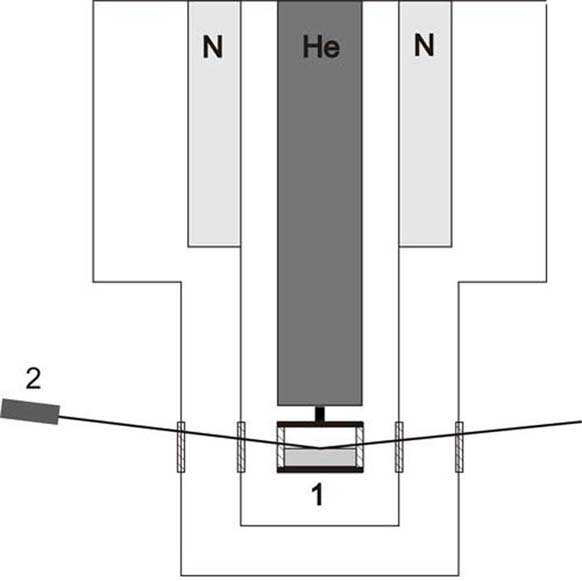
\includegraphics [scale=0.2] {article1/kriostat.jpg} \\ а)
  \end{minipage}
 \hfill
  \begin{minipage}[ht]{0.48\linewidth}
  \center
  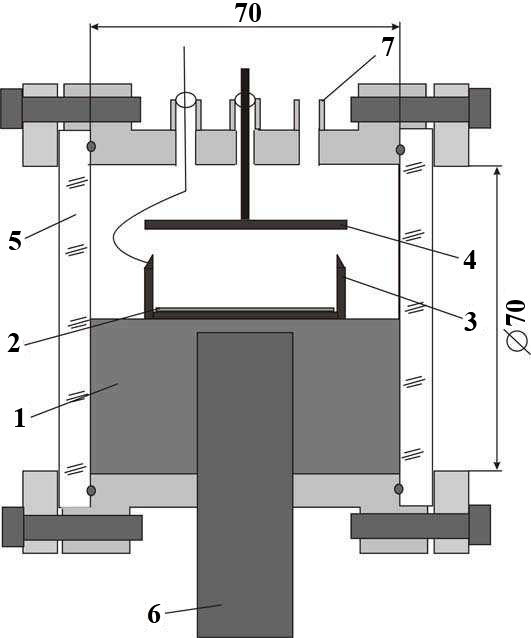
\includegraphics [scale=0.2] {article1/cell.jpg} \\ б)
   \end{minipage}
   \caption{  
   %а) Схематичная конструкция криостата. 1 – экспериментальная ячейка, 2 – лазер.   
  %б) Схематичная конструкция экспериментальной ячейки.  1 – текстолитовый брусок, 2 – радиоактивная мишень, 3 – медный контейнер, 4 – верхняя обкладка конденсатора, 5 – кварцевое окно, 6 - медный хладопровод, 7 – капилляр для набора водорода.
а) Конструкция криостата. б) Конструкция экспериментальной ячейки.
  } 
 
\label{img:cryostat} 
 
\end{figure}

Экспериментальная установка состоит из гелиевого криостата (рис.~\ref{img:cryostat}а), в вакуумной полости которого расположена оптическая ячейка (рис.~\ref{img:cryostat}б), системы возбуждения колебаний на поверхности жидкого водорода и оптической системы их регистрации. Жидкий водород конденсируется в цилиндрическую ячейку диаметром 60 мм и глубиной 6 мм. Радиоактивная мишень (молибденовая пластина, покрытая слоем тритида титана), расположенная на дне стакана, ионизирует жидкий водород. Колебания на заряженной поверхности жидкости возбуждаются переменным электрическим полем. В экспериментах в качестве переменного возбуждающего напряжения были использованы низкочастотные случайные сигналы, сосредоточенные в полосе частот 39-103 Гц.  Средний квадрат возбуждающего напряжения менялся от $V_p$ = 0 В, т.е. отсутствие накачки, до $V_p$ = 30 В


Для регистрации волн на поверхности жидкости использовался метод отраженного лазерного луча \cite{Brazhnikov_IET} в режиме "широкого"{} луча. При этом квадрат Фурье образа сигнала, принятого фотодетектором после отражения от поверхности жидкости, $P_\omega^2$ будет пропорционален Фурье образу парной корреляционной функции отклонения поверхности от положения равновесия $I(\omega)$.

\begin{figure}[ht] 
 \begin{minipage}[ht]{0.48\linewidth}
   \center
   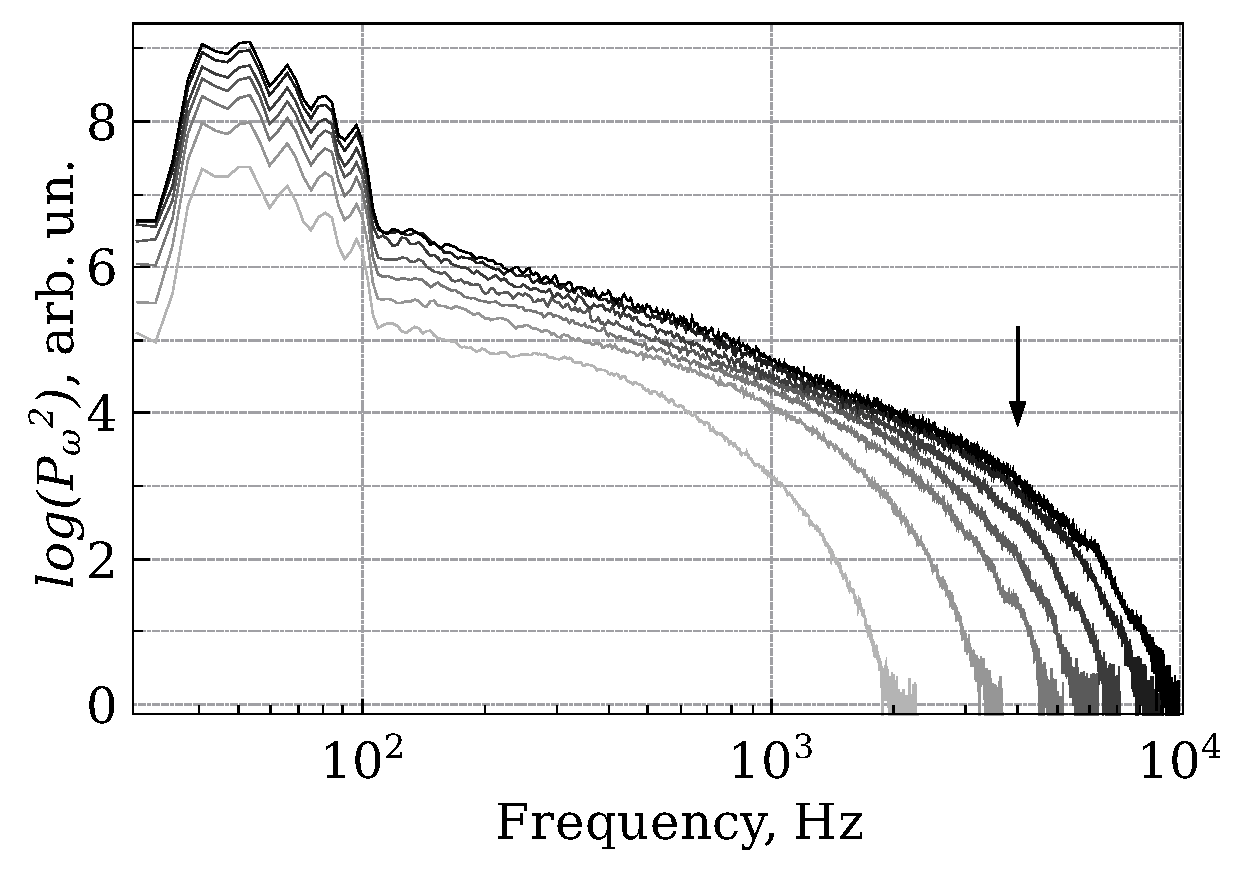
\includegraphics [scale=.275] {article1/spectra_dlog.eps} \\ а)
 \end{minipage}
 \hfill
 \begin{minipage}[ht]{0.48\linewidth}
   \center
   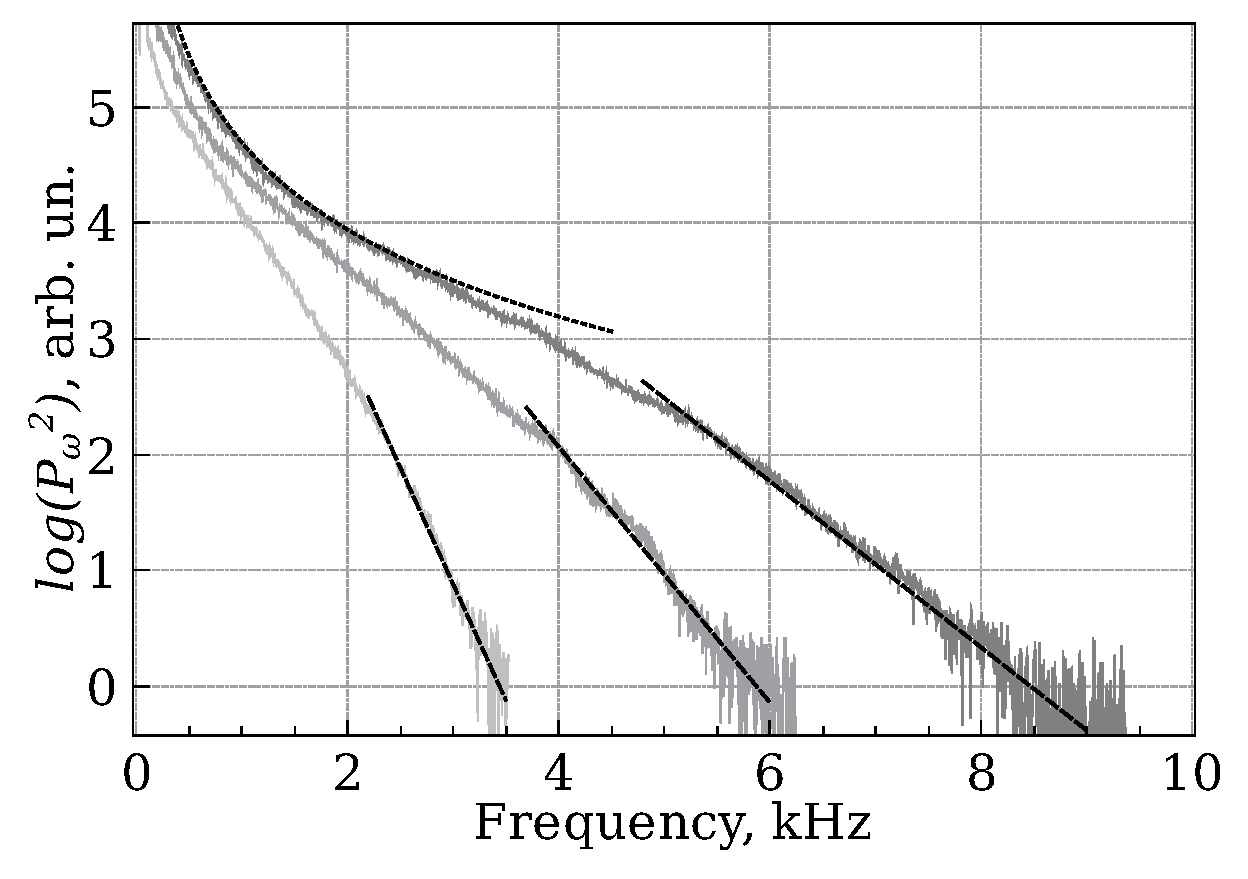
\includegraphics [scale=0.275] {article1/spectra_log.eps} \\ б)
\end{minipage}

 \caption{а) Спектры поверхностных колебаний $P^2_\omega$, возбужденных случайной силой в частотном диапазоне 39-103 Гц при разных амплитудах возбуждающей силы. Среднеквадратичное значение возбуждающего напряжения $V_P$ меняется от 4 до 30 В. Более темные линии соответствуют большей силе накачки. Стрелкой показана высокочастотная граница инерционного интервала $\omega_b \approx 4$ кГц при накачке 30 В.
  б)Спектры $P^2_\omega$ для уровней накачки $V_p = 8$ В (светло серая линия), $16$ В (серая линия) и $26$ В (темно-серая линия) в полулогарифмическом масштабе. Линией из точек показан степенной закон $\sim \omega^{-2.8}$, пунктирной линией - подгонка функцией $ \sim e^{-\omega/\omega_d}$. $\omega_d$ примерно равен 0.2, 0.4 и 0.6 кГц для $V_p$ = 8, 16 и 26 В соответственно.} 
 \label{img:hydr_specrta_dlog} 
\end{figure}

На Фурье-спек­трах отраженной энергии лазерного луча $P_\omega^2$ при разных амплитудах воз­буждающей силы видно (см. рис.~\ref{img:hydr_specrta_dlog}а), что ширина инерционного интервала зависит от амплитуды накачки. Увеличение силы накачки приводит к уширению инерционного интервала, высокочастотная граница инерционного интервала $\omega_b$ смещается к высоким частотам. 



Турбулентные спектры, построенные в полулогарифмическом масштабе (см. рис.~\ref{img:hydr_specrta_dlog}б), показывают, что распределение энергии в диссипативной области близко к экспоненциальному $P_\omega^2 \sim e^{-\omega/ \omega_d}$, причем характерная частота $\omega_d$ растет с увеличение амплитуды.

%\begin{figure}[ht] 
% \center
% 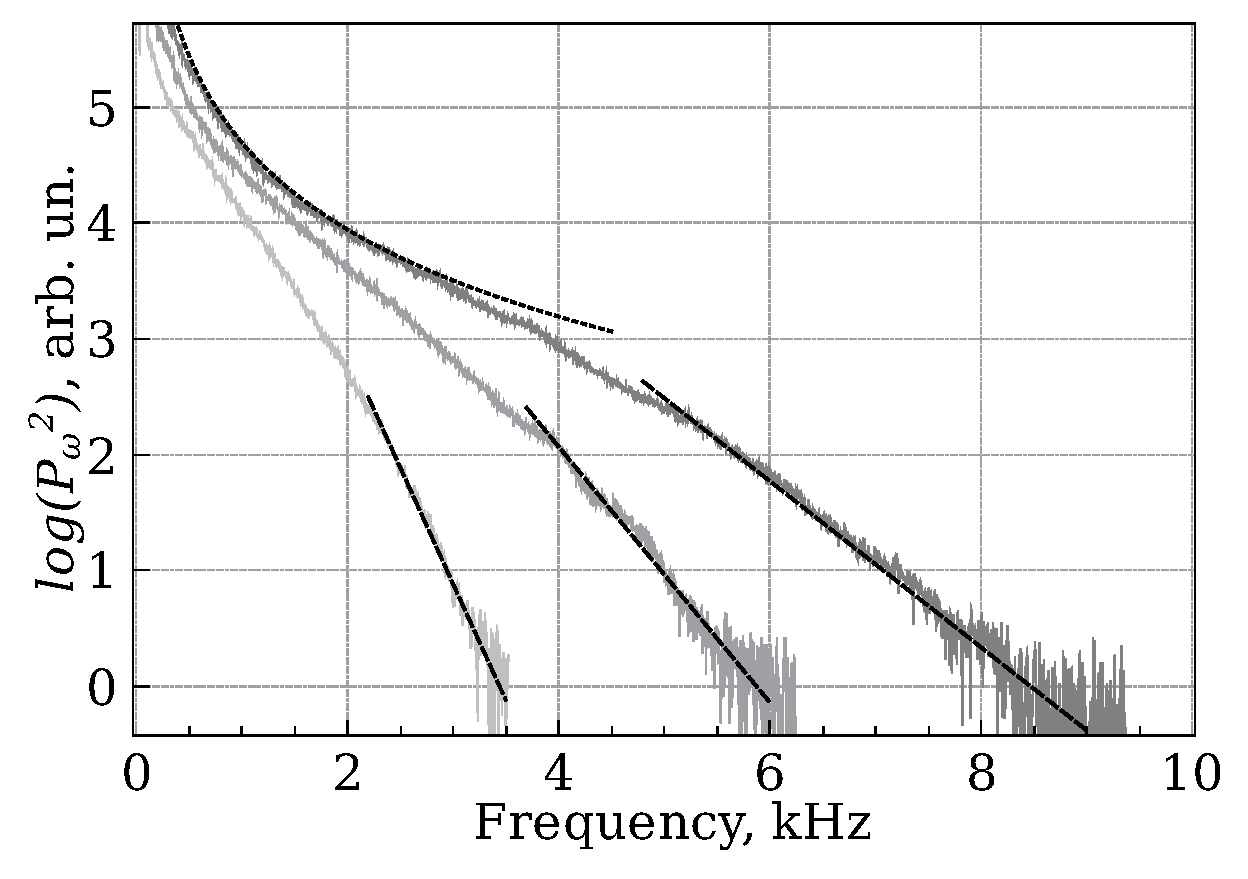
\includegraphics [scale=0.3] {article1/spectra_log.eps}
% \caption{Спектры $P^2_\omega$ для уровней накачки $V_p = 8$ В (светло серая линия), $16$ В (серая линия) и $26$ В (темно-серая линия) в полулогарифмическом масштабе. Линией из точек показан степенной закон $\sim \omega^{-2.8}$, пунктирной линией - подгонка функцией $ \sim e^{-\omega/\omega_d}$. $\omega_d$ примерно равен 0.2, 0.4 и 0.6 кГц для $V_p$ = 8, 16 и 26 В соответственно.} 
% \label{img:hydr_specrta_log} 
%\end{figure}

Для измерения уровня возбуждения использовался отклик поверхности $\eta_0$ , а именно абсолютное значение $P_\omega$ на частоте 53 Гц (положение максимума распределения $P_\omega^2$ внутри области накачки). Величина $\eta_0$ прямо пропорциональна средней высоте волны на той же самой частоте. На рис.~\ref{img:hydr_wd}  показано, что зависимость граничной частоты от значения амплитуды волны может быть описана степенным законом $\omega_d(\eta_0) \sim \eta_0^m$ со значение показателя $m = 0.85 \pm 0.05$, в то время как теория слабой волновой турбулентности предлагает значение $m = -12/5$. Стоит отметить, что подгонка экспоненциальных спектров с помощью "квазипланковского"{} распределения с малым ненулевым $s$ ($\vert s \vert \leq 2$) слабо влияет на полученный параметр $\omega_d$ (изменение менее 20\%). Эта поправка не изменит показатель степени $m$ в пределах погрешности.
\begin{figure}[ht] 
 \center
 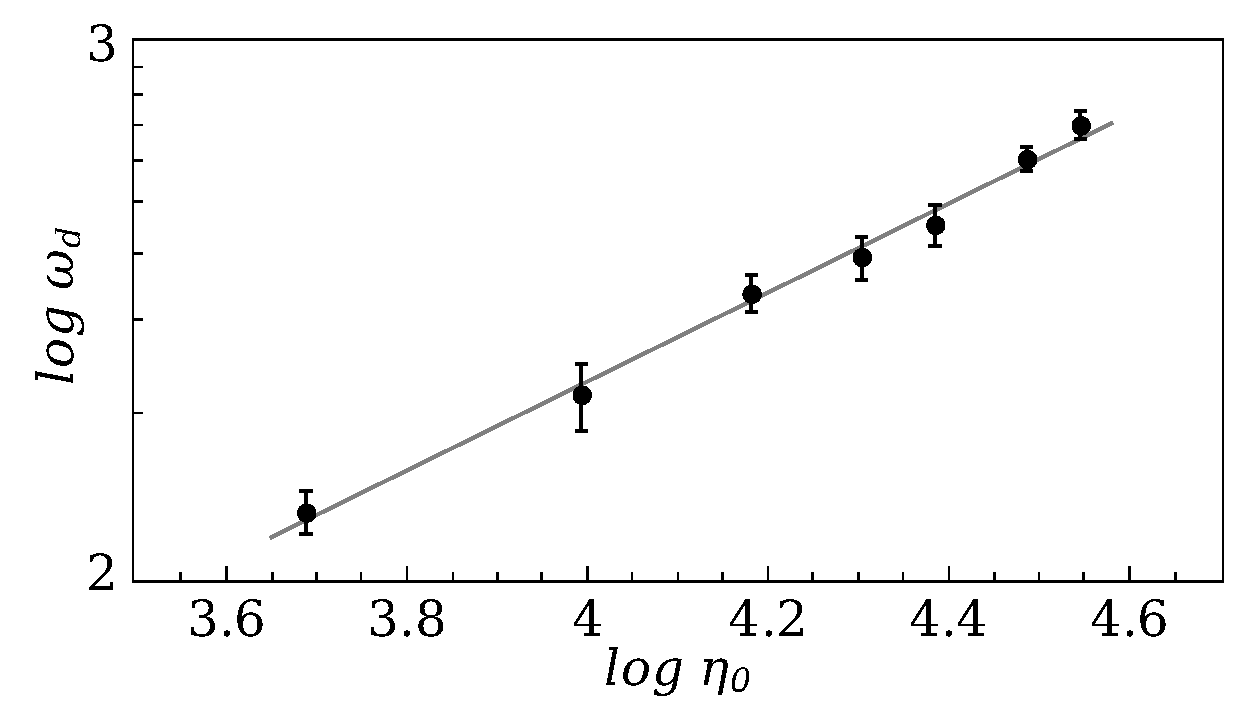
\includegraphics [scale=0.35] {article1/wd.eps}
 \caption{
 Зависимость частоты вязкого затухания диссипативной области $\omega_d$ (черные точки) от средней высоты низкочастотной волны $\eta_0$, сплошная линия - подгонка функцией $\eta_0^{0.85}$. }
 \label{img:hydr_wd} 
\end{figure}
Таким образом можно сделать выводы, что:

 - впервые наблюден переход от степенного спектра Колмогова-Захарова
в инерционном интервале к "квазипланковскому"{} распределению $\omega^{-s} e^{-\omega/\omega_d}$ в области диссипации энергии в турбулентном распределении системы капил­лярных волн;

- экспоненциальный спад в области диссипации $-\omega/ \omega_d \gg 1$ соответствует теоретическому ожиданию и качественно соответствует численным вычислениям \cite{Ryzhenkova1990}.
 
- граница вязкого затухания $\omega_d$ растет с увеличением амплитуды накачки и зависит от средней высоты волны $\eta_0$ на частоте накачки как $\omega_d \sim \eta_0^{0.85 \pm 0.05}$. Однако наблюденная зависимость отличается от теоретически ожидаемой, показатель степени почти в три раза больше предсказанного значе­ния.

\underline{\textbf{Вторая глава}} посвящена экспериментальному изучению особенностей распределения энергии в диссипативной области стационарного турбулентного спектра в системе капиллярных волн на поверхности воды, а также положению высокочастотной границы инерционного интервала в зависимости от амплитуды и типа накачки.

Экспериментальные ячейки имели форму стакана с кругом диаметром от 65 до 130 мм или прямоугольником со сторонами 49 $\times$ 50 мм в основании и глубиной 10 мм. Колебания на поверхности воды возбуждаются вертикальными колебаниями экспериментальной ячейки. Методика регистрации была такая же как в экспериментах с жидким водородом. Использовались следующие виды накачек: монохроматическая на резонансной частоте, узкополосная с шириной полосы около 1 Гц и широкополосная в диапазоне 30–50 Гц. Под амплитудой накачки А в случае монохроматического возбуждения понимается амплитуда электрического сигнала, подаваемого на виброплатформу. В случае узкополосной или широкополосной накачки за амплитуду А принимается среднеквадратичное значение электрического сигнала, подаваемого на виброплатформу.

\begin{figure}[ht]
 \begin{minipage}[ht]{0.49\linewidth}
 \center{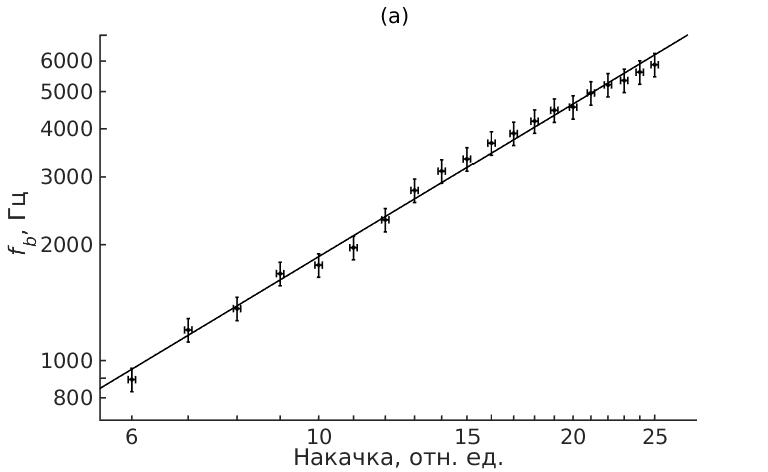
\includegraphics[width=1\linewidth]{article2/pic_06a.jpg} \\ а)}
 \end{minipage}
 \hfill
 \begin{minipage}[ht]{0.49\linewidth}
 \center{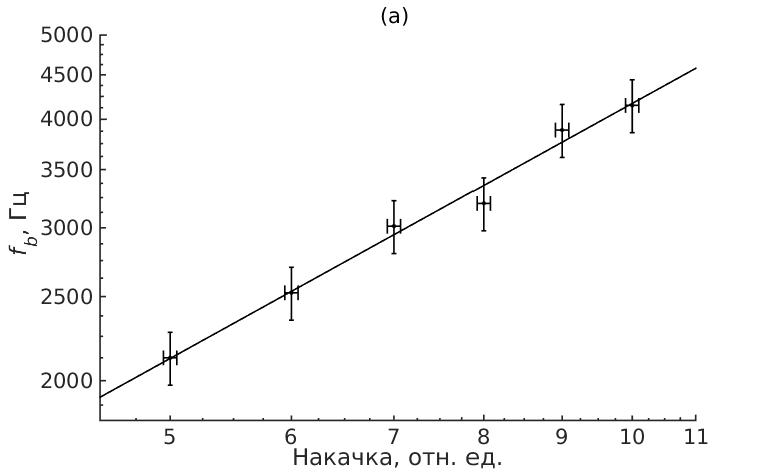
\includegraphics[width=1\linewidth]{article2/pic_07a.jpg} \\ б)}
 \end{minipage}
 \caption{Зависимость высокочастотного края инерционного интервала $f_b$ от амплитуды возбуждающей силы в цилиндрических ячейках диаметром 65 мм, при а) монохроматической накачке на частоте $f_p$ = 45.5 Гц. Прямая линия соответствует степенной зависимости частоты от амплитуды накачки с показателем степени $\beta = 1.32$
 б) широкополосной накачки в интервале 30–50 Гц. Прямая линия соответствует степенной зависимости частоты от амплитуды накачки с показателем степени $\beta = 0.97$}

 \label{img:water_fb_65} 
\end{figure}
Экспериментальное исследование дает степенную зависимость положения границы инерционного интервала в зависимости от амплитуды накачки для разных типов накачки $f_b \sim A^\beta$ (см. рис.~\ref{img:water_fb_65}).

 Так же степенным образом зависит от амплитуды накачки характерная частота в показателе экспоненты, описывающей затухание распределения энергии в диссипативной области турбулентного спектра $f_d \sim A^\beta$ (см. рис.~\ref{img:water_fd_65}).



При монохроматической накачке получаются зависимости: $f_b \sim A^{1.23 \pm 0.10}$,  $f_d \sim A^{1.28 \pm 0.10}$. Видно, что показатели степени близки к теоретическому значению для монохроматической накачки $\beta = -4/3$.

Для широкополосной накачки получаются зависимости: $f_b \sim A^{0.96 \pm 0.02}$,  $f_d \sim A^{1.13 \pm 0.00}$, отличающиеся от теоретического значению $\beta = -12/5$.

Таким образом можно сделать выводы:

-экспериментально показано, что при возбуждении турбулентного состояния на поверхности воды монохроматической или широкополосной накачкой частота высокочастотного края инерционного интервала и характерная частота вязкого затухания каскада $P_\omega^2$ в диссипативной области отличаются в несколько раз и качественно одинаково повышаются с ростом амплитуды накачки по степенному закону с показателем степени, близким к теоретически оцененному значению для монохроматического возбуждения;

- в случае широкополосной накачки наблюдается значительное расхождение между экспериментальными и теоретически оцененными значениями показателя $\beta$; 

- показано, что значения показателя степени слабо зависит от геометрии экспериментальной ячейки.

\begin{figure}[ht]
 \begin{minipage}[ht]{0.49\linewidth}
 \center{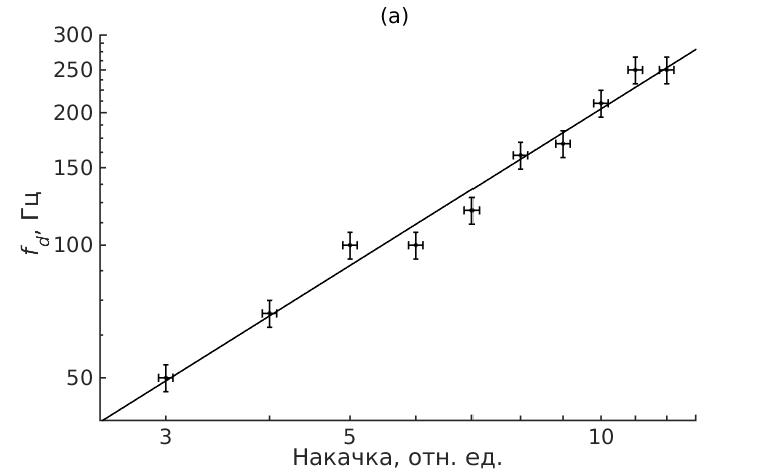
\includegraphics[width=1\linewidth]{article2/pic_09a.jpg} \\ а)}
 \end{minipage}
 \hfill
 \begin{minipage}[ht]{0.49\linewidth}
 \center{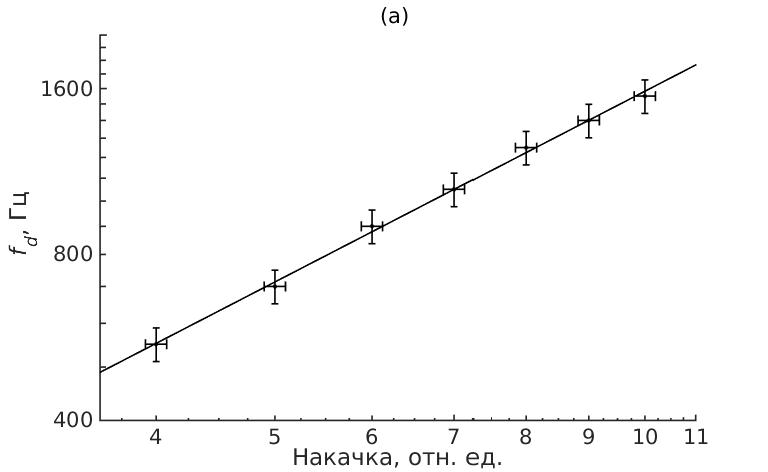
\includegraphics[width=1\linewidth]{article2/pic_11a.jpg} \\ б)}
 \end{minipage}
 \caption{Зависимость характерной частоты $f_d$ от амплитуды возбуждающей силы в ячейке диаметром 65 мм при а) монохроматической накачке на частоте 45.5 Гц. Прямая линия соответствует степенной зависимости частоты от амплитуды накачки с показателем степени $\beta = 1.18$.
 б) широкополосной накачке на частотах от 30 до 50 Гц в ячейке диаметром 65; Прямая линия соответствует степенной зависимости частоты от амплитуды накачки с показателем степени $\beta = 1.15$.}
 \label{img:water_fd_65} 
\end{figure}


\underline{\textbf{Третья глава}} посвящена исследованию генерации вихревого движения из-за взаимодействия нелинейных капиллярных волн, распространяющихся под углом друг к другу, на поверхности воды.

Экспериментальная установка
%(см. рис.~\ref{img:setup50})
 состоит из виброплатформы, на которой установлена ячейка цилиндрической (диаметр 65 мм) или прямоугольной (49 $\times$ 50 мм$^2$) формы глубиной 10 мм. В экспериментальную ячейку налита дистиллированная воды. Для декорирования вихревного движения на поверхность воды насыпаны полые алюмосиликатные микросферы или частички полиамида PA-12. Над ячейкой расположена камера, которая снимает движение частичек на поверхности воды. Полученное видео разбивается на кадры и для каждой последовательной пары кадров с помощью пакета PIVlab для Matlab \cite{PIVlab} вычисляется поле скорости на поверхности жидкости.

%\begin{figure}[ht] 
% \center
% 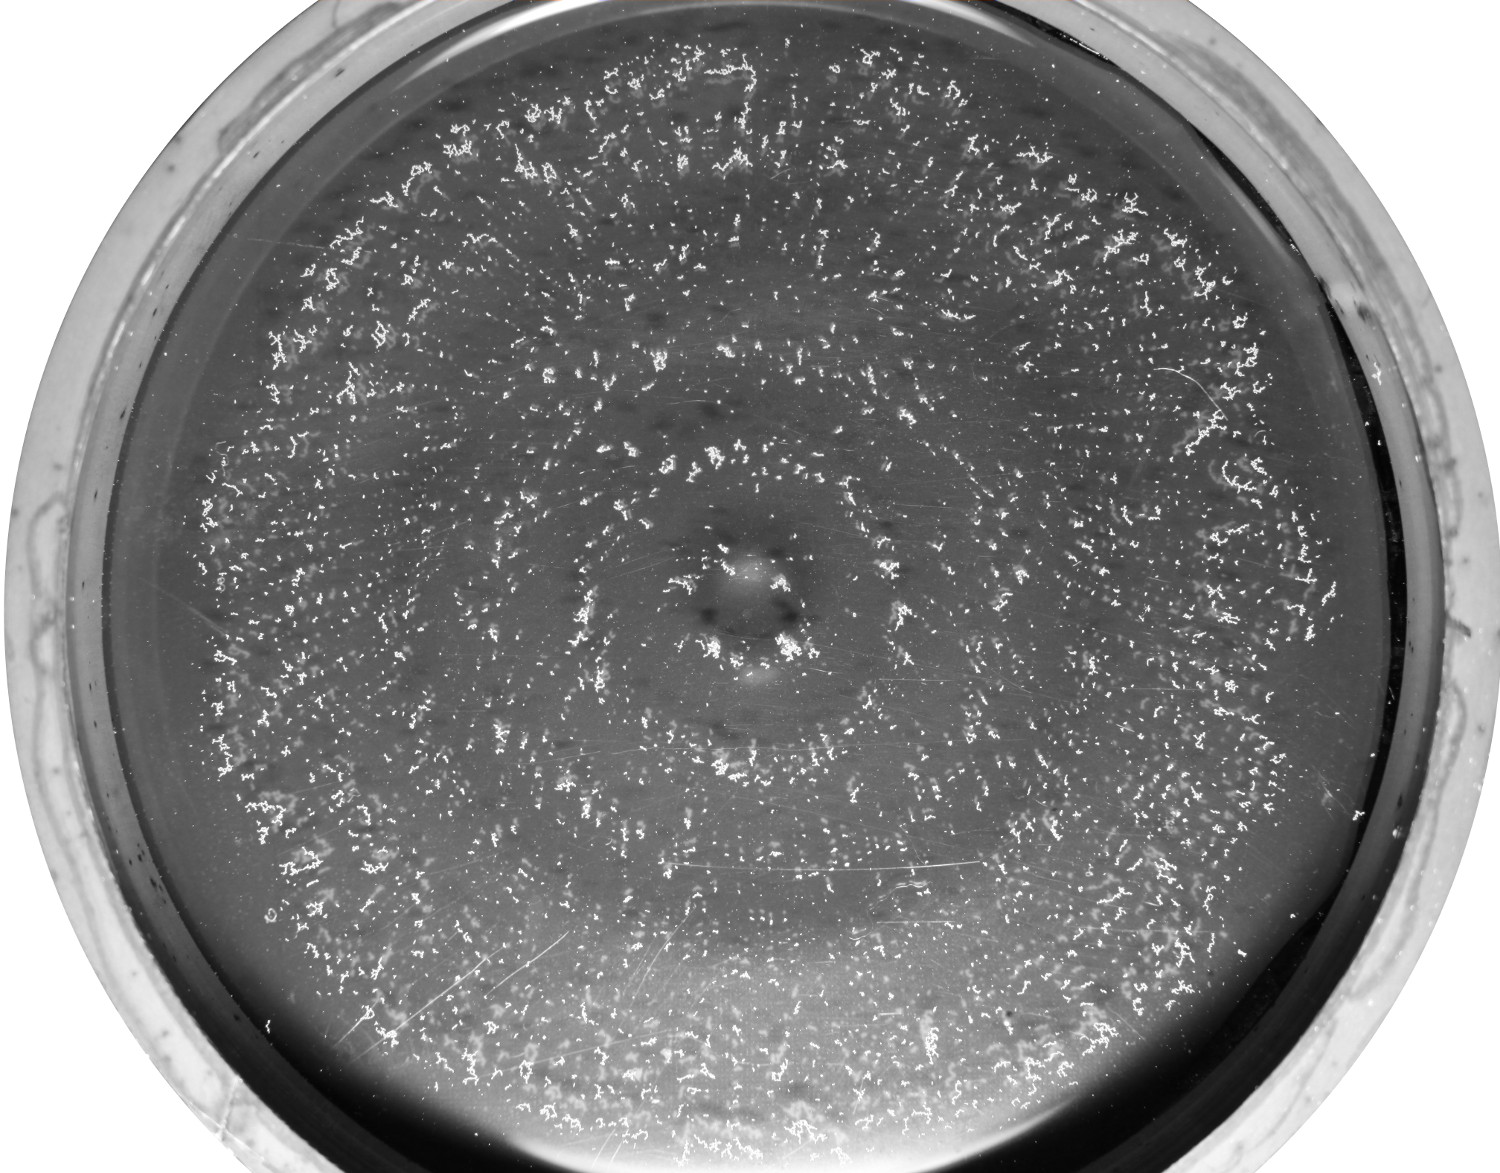
\includegraphics [scale=1] {article4/pic_01.jpg}
% \caption{Экспериментальная установка для регистрации вихревых движений на поверхности воды. а) Схема установки: 1 - ячейка, 2 - вода, 3 - виброплатформа, 4 - фотоаппарат, 5 - фотовспышка. b) Вогнутый или выпуклый мениск формируется на краю стенок в зависимости от количества воды, используемой для заполнения сосуда. с) Конфигурация водяного мениска в квадратной ячейке, имеющей стенки разной высоты, предназначенная для подавления генерации волн от пары соседних стенок. Стрелки показывают направление распространения волны.} 
%  \label{img:setup50} 
%\end{figure}
При возбуждении волн радиальной моды в цилиндрической ячейке вихрей на поверхности воды не возникает (см рис.~\ref{img:vort_st}а). Изменение симметрии ячейки путем добавления двух столбушков приводит к появлению вихревой структуры  (см. рис.~\ref{img:vort_st}б). При возбуждении угловой моды в цилиндрической ячейке или двух перпендикулярных волн в прямоугольной ячейке на поверхности воды также возникает вихревая структура, напоминающая структуру волн (см. рис.~\ref{img:vort_chess}а). Таким образом можно сделать предположение, что вихревое движение возникает за счет взаимодействия волн, распространяющихся под углом друг к другу.

\begin{figure}[ht]
 \begin{minipage}[ht]{0.49\linewidth}
 \center{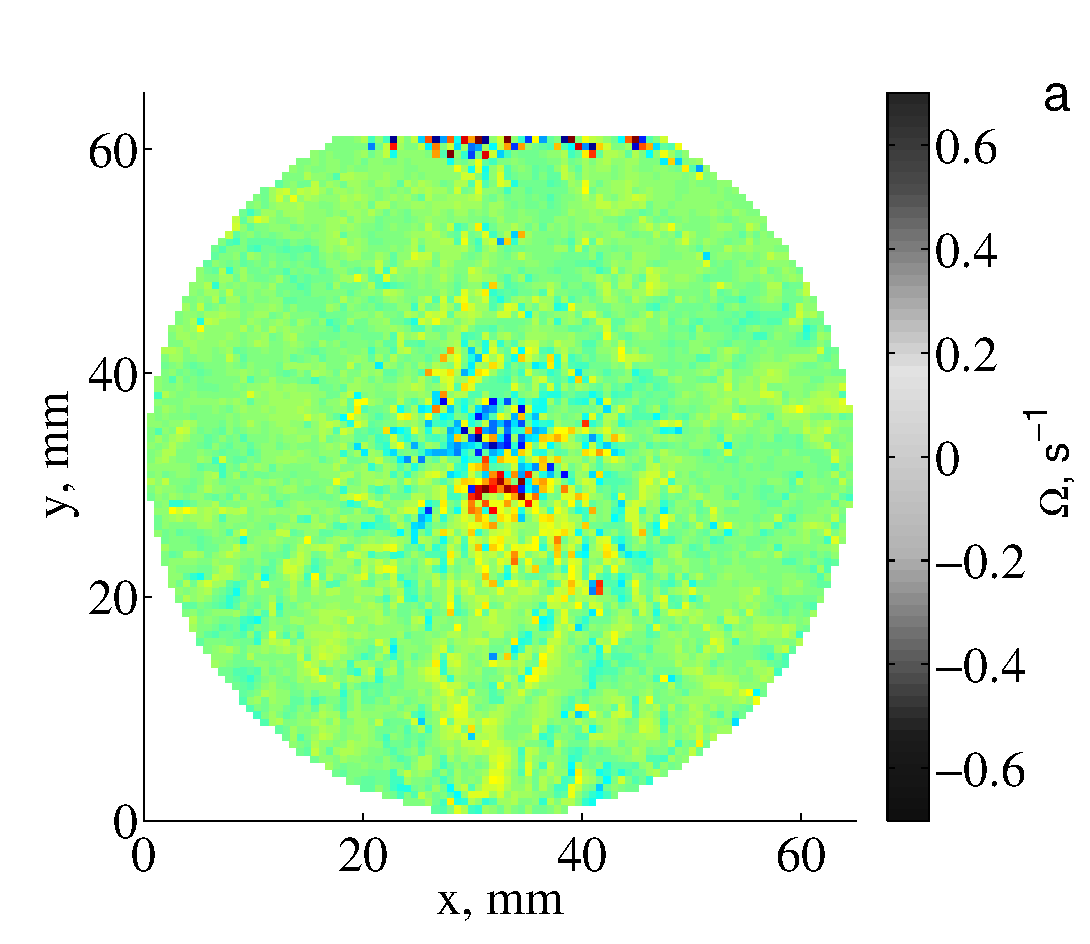
\includegraphics[width=1\linewidth]{article3/pic_06a.eps} \\ а)}
 \end{minipage}
 \hfill
 \begin{minipage}[ht]{0.49\linewidth}
 \center{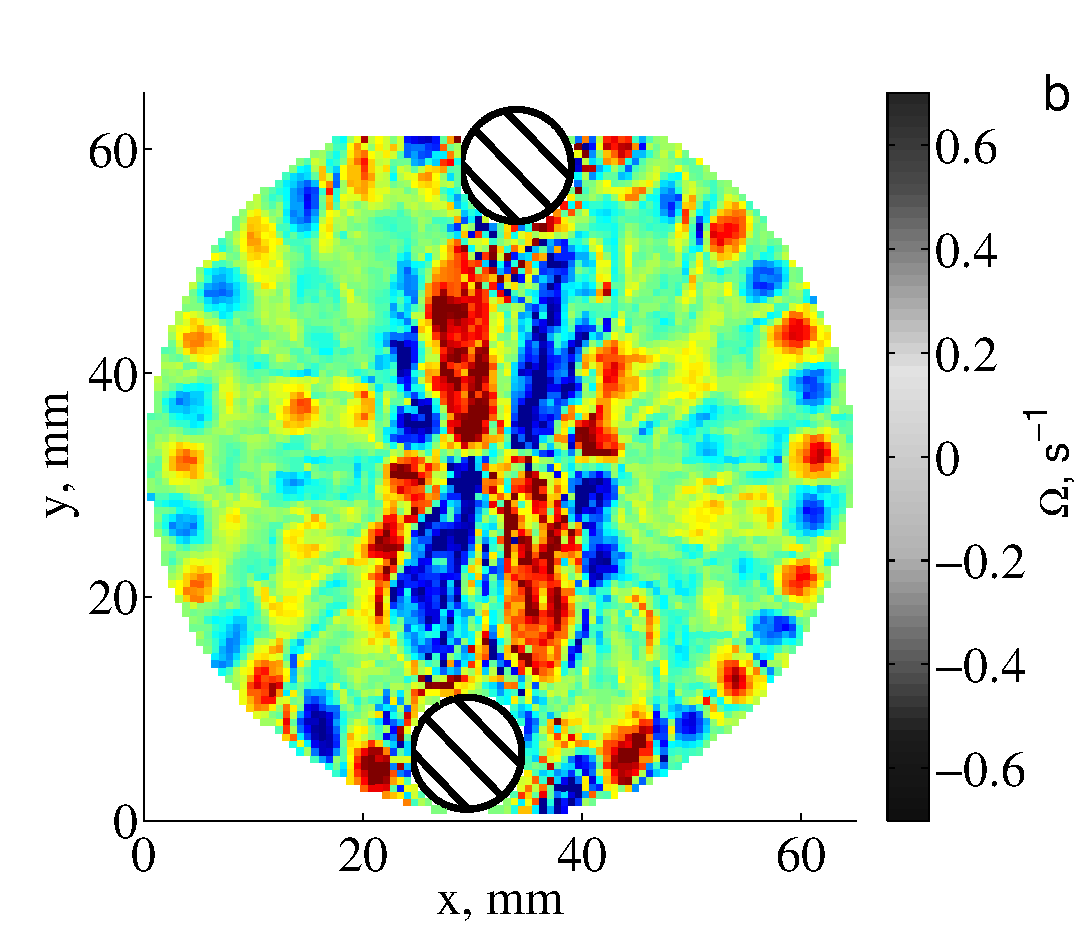
\includegraphics[width=1\linewidth]{article3/pic_06b.eps} \\ б)}
 \end{minipage}
 \caption{Поле завихренности $\Omega$ в цилиндрическом сосуде, в котором установлены два пластиковых столбика. На вставке – завихренность до установки столбиков. Цветовая шкала для завихренности общая.}
 \label{img:vort_st} 
\end{figure}

В работе \cite{F6} была построена теоретическая модель генерации вихревого движения в случае взаимно перпендикулярных стоячих волн и в случае взаимно перпендикулярных бегущих волн.

\begin{figure}[ht] 
 \begin{minipage}[ht]{0.49\linewidth}
  \center
  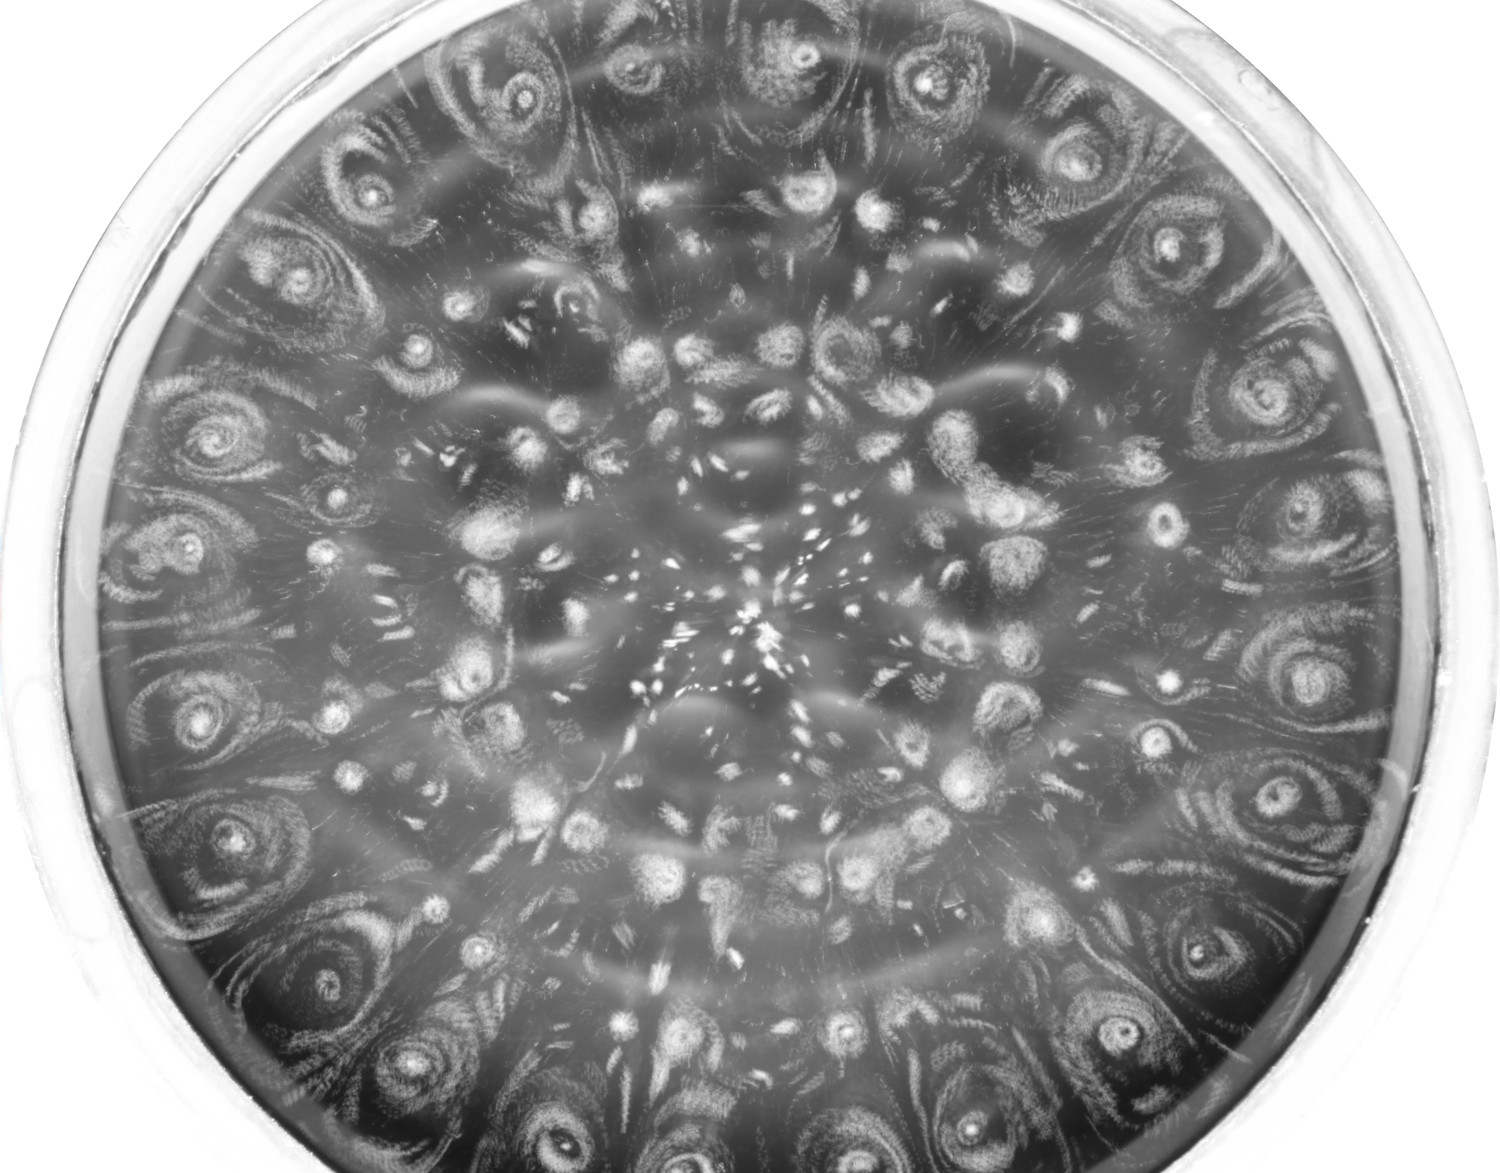
\includegraphics [scale=.38] {article4/pic_02.eps}
 \end{minipage}
 \hfill
 \begin{minipage}[ht]{0.49\linewidth}
  \center
  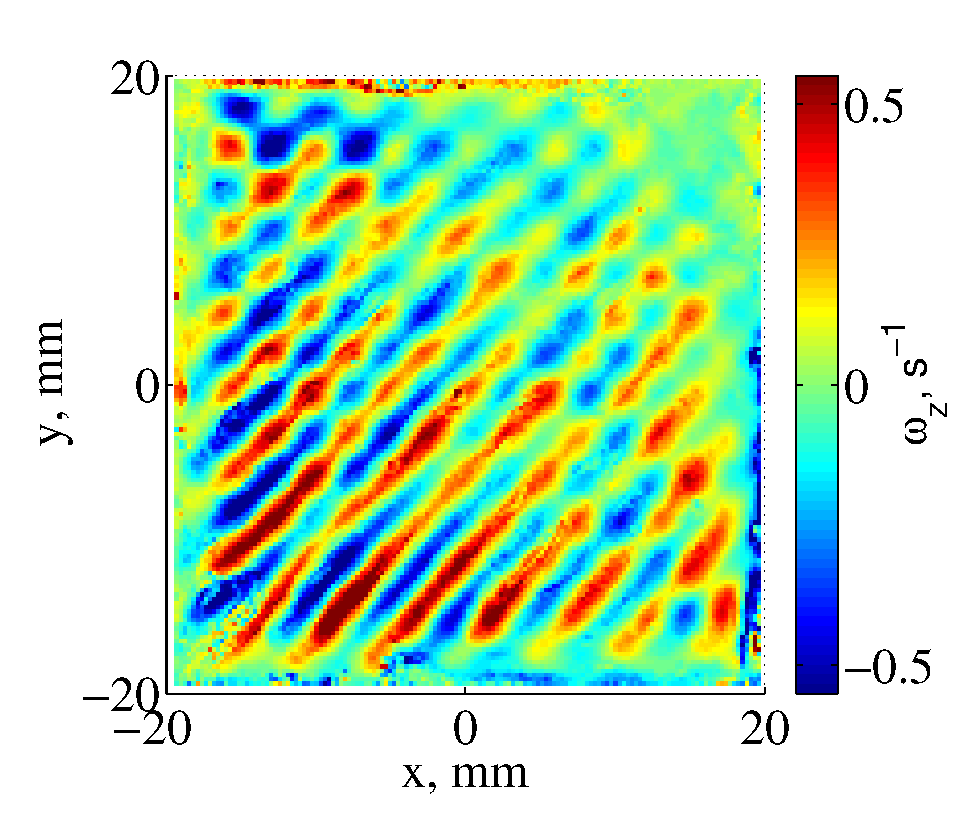
\includegraphics [scale=.38] {article4/pic_03.eps}
 \end{minipage}  
 \caption{а) Завихренность в ячейке 50 x 49 мм$^2$ при возбуждении поверхностных волн с частотой 42.7 Гц. Наблюдается шахматноподобный паттерн поля завихренности соответствующий теоретическому выражению (\ref{eq:vortStand}). Периоды решетки в $X$ и $Y$ направлениях равны длине волны.
 б) Завихренность в ячейке 40 х 40 мм $^2$ при возбуждении поверхностных волн с частотой 54 Гц. Две стенки ячейки соответствующие левой и нижней части рисунка немного ниже, чем остальные станки. Уровень воды скорректирован, чтобы в основном возникало две бегущие волны от более низких стенок. Знакопеременные полосы положительной и отрицательной завихренности, направленные параллельно диагонали квадратной ячейки, согласуются с теоретическим выражением (\ref{eq:vortRun}).} 
 \label{img:vort_chess} 
\end{figure}

В первом случае теоретическая модель построена для двух стоячих волн, описываемых уравнением:

\begin{equation}
\label{eq:waveStand}
h(x, y, t) = H_1 sin(kx)cos(\omega t)+H_2 sin(ky)cos(\omega t+ \phi),
\end{equation}
где $\phi$ разность фаз между стоячими волнами в разных направлениях.

Согласно предсказанию построенной модели завихренность на поверхности жидкости в стационарном режиме будет описываться выражением:

\begin{equation}
\label{eq:vortStand}
\Omega = -(1 + \sqrt{2}) H_1 H_2 \omega k^2 sin(kx)sin(ky) sin \phi
\end{equation}

Эксперимент по генерации завихренности на поверхности воды в прямоугольной ячейке размером 49 $\times$ 50 мм$^2$ показывает пространственное распределение завихренности качественно совпадающее с формулой (\ref{eq:vortStand}) (см. рис.~\ref{img:vort_chess}а). 


Серия экспериментов, проведенных при разном уровне накачки, показывает, что амплитуда завихренности решетки вихрей в зависит от амплитуды волны квадратичным образом (рис.~\ref{img:vort_ampl}), что хорошо согласуется с формулой (\ref{eq:vortStand}).

\begin{figure}[ht] 
 \center
 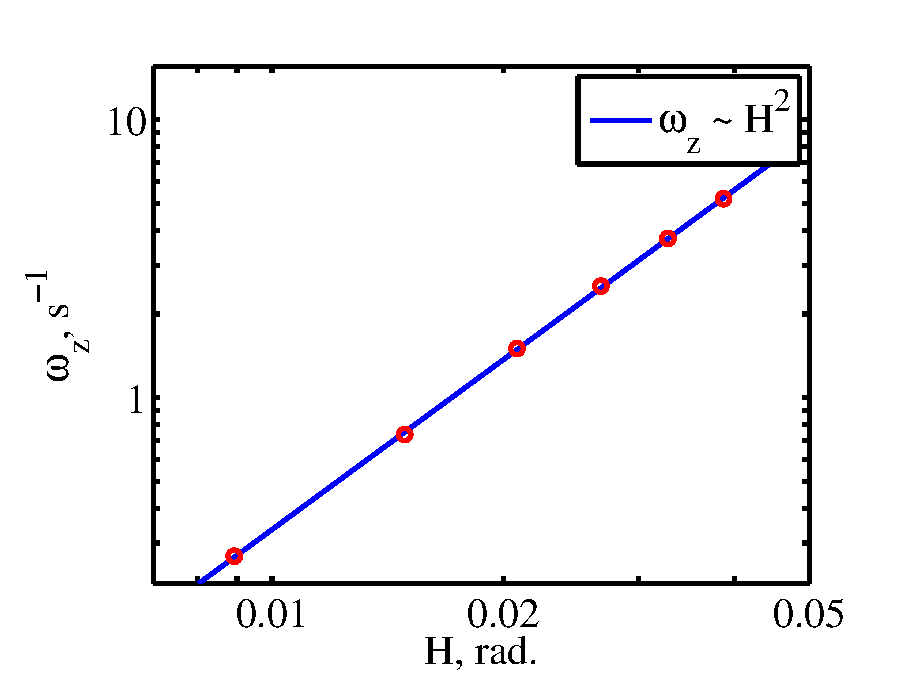
\includegraphics [scale=.35] {article4/pic_04.eps}
 \caption{Амплитуда завихренности для различных амплитуд накачки в ячейке 50 x 49 мм$^2$, где возбуждаются поверхностные волны с частотой 42.7 Гц, построенная в зависимости от амплитуды накачки. Линия соответствует зависимости $\Omega \sim H^2$.} 
 \label{img:vort_ampl} 
\end{figure}

Так же теоретическая модель построена для двух перпендикулярных бегущих волн, описываемых уравнением:

\begin{equation}
\label{eq:waveRun}
h(x, y, t) = H_1 sin(kx-\omega t)+H_2 sin(ky-\omega t)
\end{equation}

В этом случае завихренность на поверхности жидкости в стационарном режиме будет описываться выражением:

\begin{equation}
 \label{eq:vortRun}
\Omega = -(1 + \sqrt{2})H_1 H_2 \omega k^2 sin(kx-ky)
\end{equation}
Эксперимент по генерации завихренности на поверхности воды в квадратной ячейке размером 40 $\times$ 40 мм$^2$ показывает пространственное распределение завихренности качественно совпадающее с формулой (\ref{eq:vortRun}) (см. рис.~\ref{img:vort_chess}б). 

Таким образом можно сделать выводы:

 - открыт новый механизм генерации поверхностной завихренности, связан­ный с взаимодействием нелинейных поверхностных волн в тонком вязким под­слоем;

 - экспериментально наблюдена квадратичная зависимость модуля завих­ренности от угловой амплитуды волны;
 
 - наблюденные экспериментальные рас­пределения вихревого движения, генерируемого взаимно перпендикулярными как стоячими, так и бегущими волнами, качественно хорошо согласуются с тео­ретической моделью.


%Увеличивая амплитуду вертикальных колебаний ячейки можно достичь порога неустойчивости Фарадея. Значительно выше порога, поверхностные вол­ны весьма интенсивны, что приводит к интенсивным вихревым движениям по­верхности жидкости, для которых угловая амплитуда приближается к 1. Тогда взаимодействие вихревых движений друг с другом становится значительным [48], что приводит, в частности, к образованию каскада энергии [27]. Результа­ты наших теоретических и экспериментальных исследований позволяют лучше понять это явление и разработать количественную основу для него.

\underline{\textbf{Четвертая глава}} посвящена исследованию генерации вихревого движения из-за взаимодействия нелинейных гравитационных волн, распространяющихся под углом друг к другу, на поверхности воды.

\begin{figure}[ht]
 \begin{minipage}[ht]{0.49\linewidth}
 \center{\includegraphics[width=.82\linewidth]{article5/pic_02a.eps} \\ а)}
 \end{minipage}
 \hfill
 \begin{minipage}[ht]{0.49\linewidth}
 \center{\includegraphics[width=1\linewidth]{article5/pic_02b.eps} \\ б)}
 \end{minipage}
 \caption{а) Треки полиамидных частиц на поверхности воды при накачке двумя плунжерами на частоте 3\,Гц с угловой амплитудой волны в центре ванны $\mu = 0.035$ рад. б) Распределение завихренности на поверхности воды при накачке двумя плунжерами на частоте 3\,Гц. Разность фаз $\psi = 90^\circ$.}
 \label{img:vort_3Hz} 
\end{figure}
 
Экспериментальная установка состоит из ванны размером 70 $\times$ 70 см$^2$, заполненной дистиллированной водой. Глубина воды составляет 10 см. Волны на поверхности воды возбуждаются волнопродукторами - двумя перпендикулярными плунжерами совершающими вертикальные колебания по действием приводов плунжеров. В качестве плунжеров используются горизонтальные стальные полые трубки, запаянные с концов, полупогруженные в воду. Приводами плунжеров служат сабвуферы TS-W254R фирмы Pioneer номинальной мощностью 250 Вт. 


Для визуализации вихревого движения на поверхность воды насыпан порошок полиамида PA-12. Камера Canon 70D, расположенная над ванной, регистрирует движение частичек полиамида.
За счет того, что плунжеры не связаны друг с другом физически, можно устанавливать произвольную разность фаз между ними.

В экспериментах использовалась монохроматическая накачка на частотах 3,4,6 Гц.

При накачке на частоте 3 Гц (длина волны 17.5 см), на поверхности воды хорошо видна решетка вихрей с характерным размером вихря около 8 см (см рис.~\ref{img:vort_3Hz}а). Пространственное распределение завихренности в решетки вихрей, возбужденной на поверхности воды, соответствует теоретической модели.

Серия экспериментов проведенных при разном уровне накачки показывает что амплитуда завихренности решетки вихрей в зависит от амплитуды волны квадратичным образом (рис.~\ref{img:ampl_phase}а), что хорошо согласуется с формулой (\ref{eq:vortStand}).
\begin{figure}[ht]
 \begin{minipage}[ht]{0.48\linewidth}
 \center{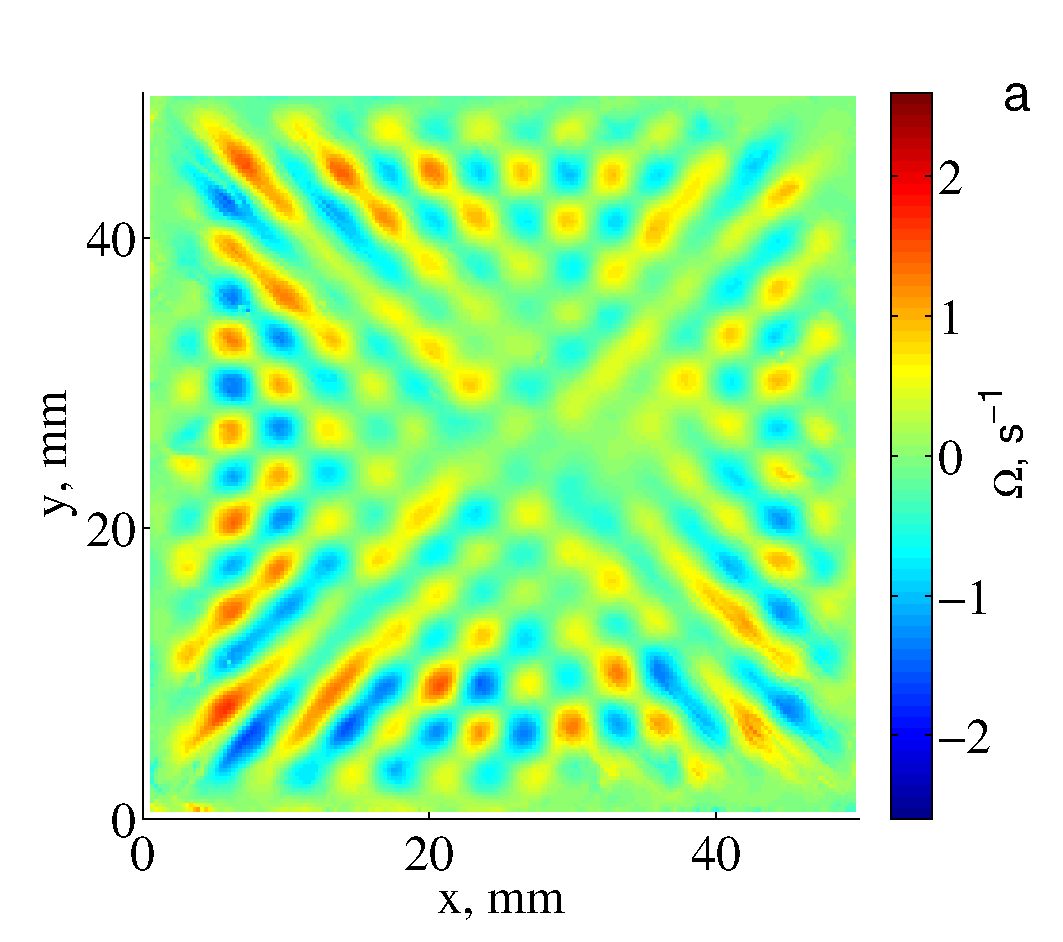
\includegraphics[width=1\linewidth]{article5/pic_03a.eps} \\ а)}
 \end{minipage}
 \hfill
 \begin{minipage}[ht]{0.48\linewidth}
 \center{\includegraphics[width=1\linewidth]{article5/pic_03b.eps} \\ б)}
 \end{minipage}
 \caption{а) Зависимость корня квадратного амплитуды завихренности $\sqrt{\Omega_0}$ на поверхности воды от угловой амплитуды волн $\mu$ при накачке двумя плунжерами на частоте 3\,Гц. Разность фаз $\psi=90^\circ$. б) Зависимость амплитуды завихренности $\Omega_0$ от разности фаз между синусоидальными сигналами, подаваемыми на волнопродукторы. Точки – эксперимент, сплошная кривая $\Omega_0 = \,0.183\, sin(\psi)$}
 \label{img:ampl_phase} 
\end{figure}
 
Эксперименты, проведенные при фиксированной амплитуде и меняющейся разности фаз в диапазоне от 0 до 180 градусов, показывают синусоидальную зависимость амплитуды решетки вихрей от амплитуды накачки (см. рис.~\ref{img:ampl_phase}б), что также хорошо согласуется с теоретической формулой (\ref{eq:vortStand}).

Однако при накачках на частотах 4 и 6 Гц на поверхности воды помимо решетки вихрей образуются крупномасштабные вихревые течения. Пример такого движения показан на рис.~\ref{img:vort_4Hz}а. На рис.~\ref{img:vort_4Hz}б показаны спектры энергии при накачке на частотах 3, 4 и 6 Гц. Видно, что при накачке на частотах 4 и 6 Гц в спектре появляются пики на малых волновых числах, что соответствует крупномасштабным течениям.
\begin{figure}[ht]
 \begin{minipage}[ht]{0.49\linewidth}
 \center{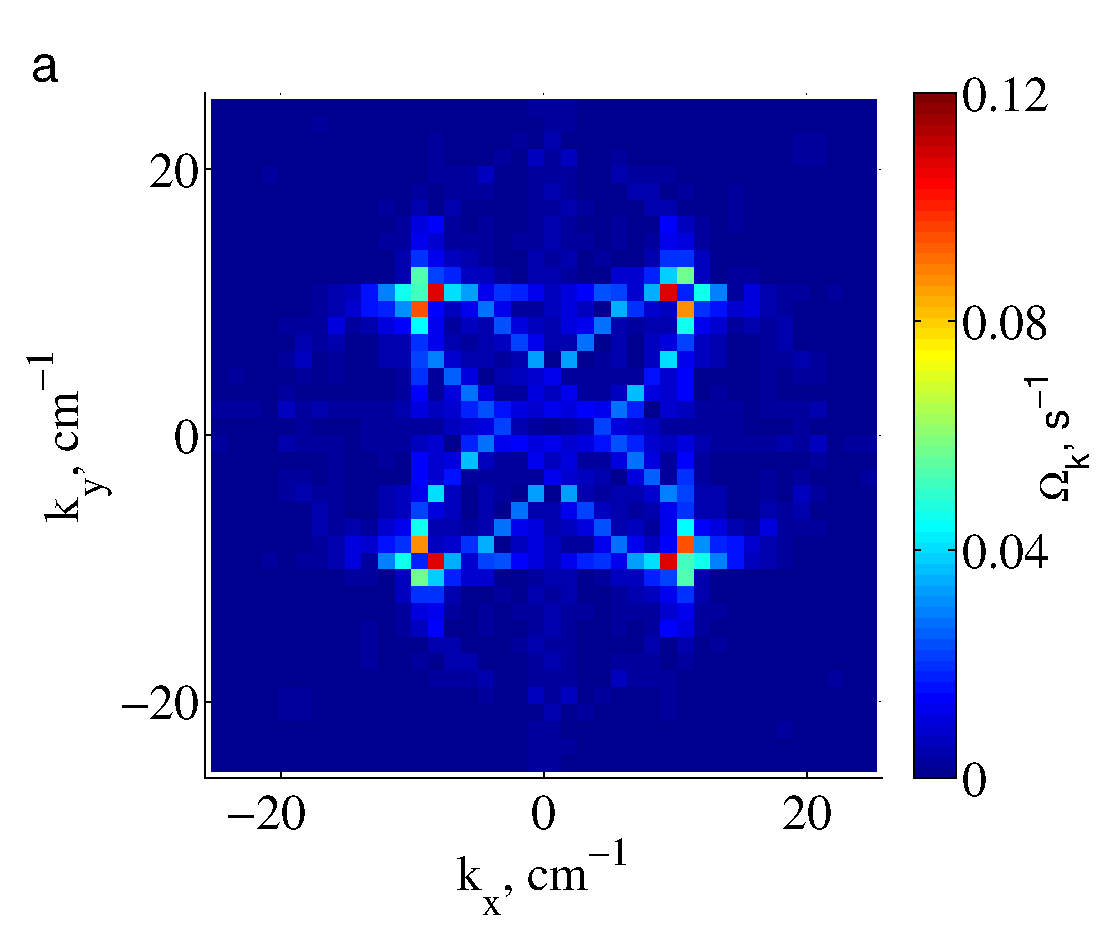
\includegraphics[scale=0.38]{article5/pic_04a.eps} \\ а)}
 \end{minipage}
 \hfill
 \begin{minipage}[ht]{0.49\linewidth}
 \center
 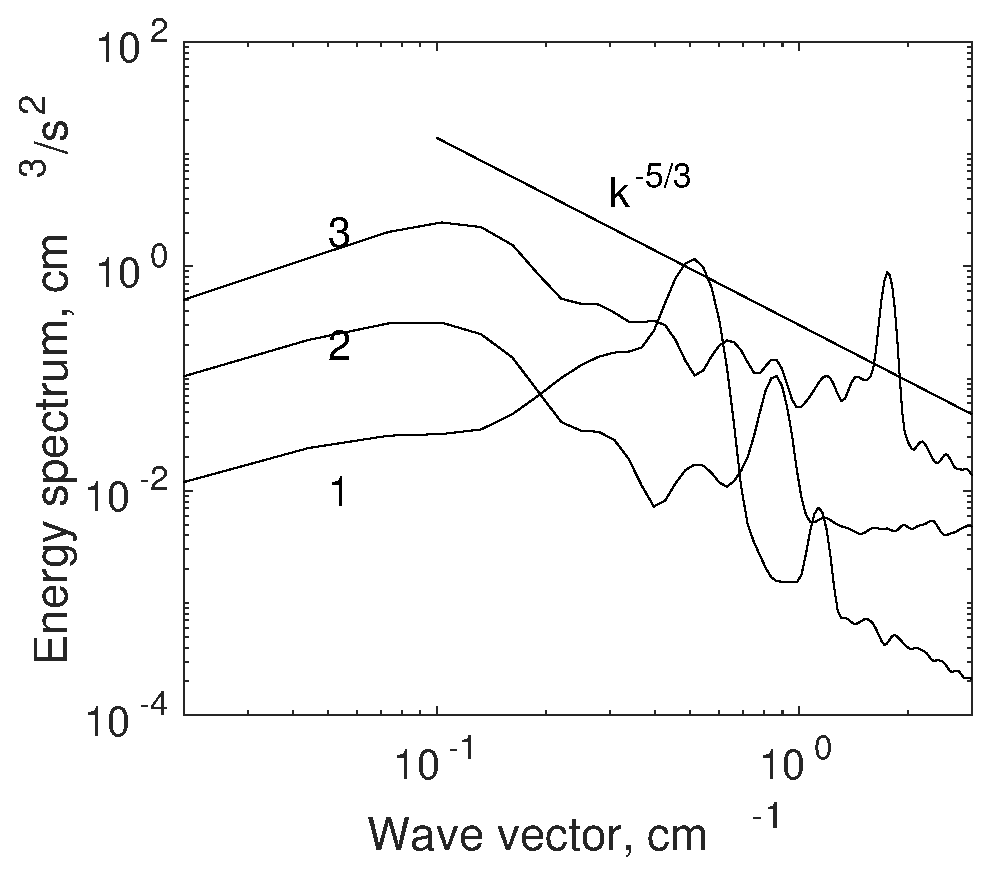
\includegraphics [scale=0.38] {article5/pic6_diss.eps}  \\ б)
 \end{minipage}
 \caption{а) Треки полиамидных частиц на поверхности воды при накачке двумя плунжерами на частоте 4\,Гц. Амплитуда волн на расстоянии 3\,см от плунжеров равна $H = 1.0 \pm 0.2$\,мм.
б) Распределение энергии $E(k)$ по волновому вектору при накачке двумя плунжерами на частоте 3\,Гц (кривая 1), 4\,Гц (кривая 2) и 6\,Гц (кривая 3).}
 \label{img:vort_4Hz} 
\end{figure}
Таким образом можно сделать выводы:

 - в данной работе впервые экспериментально показано, что завихренность,
формируемая на поверхности воды слабо нелинейными гравитационными волнами, зависит от разности их фаз и хорошо описывается выражениями, полу­ченными в работе \cite{F6}.

 - Амплитуда завихренности на поверхности квадратично зависит от амплитуды волн. Таким образом, модель генерации вихревого движения нелинейными волнами применима для описания завихренности на поверх­ности жидкости не только для волн капиллярного диапазона с длиной волны около 0.5 см, но и для гравитационных волн с длинами волн порядка 10 см.
 
 - Экспериментально наблюдена передача энергии из области накачки (масштаб решетки вихрей) в область больших масштабов. Механизм передачи энергии пока не установлен, требуются дополнительные исследования.
 
 \underline{\textbf{Пятая глава}} посвящена исследованию проникновению сгенерированной взаимодействием нелинейных волн решетки вихрей в объем жидкости.
 
Согласно построенной теоретической модели есть два механизма генерации вихревого движения волнами распространяющимися под углом друг к другу.

Первый, заключается в переносе жидкости в результате дрейфа Стокса. Согласно ему вихревое движение возникает сразу в каждой точке, где появляются волны, и исчезает сразу же как волны затухают или уходят из исследуемой области. Зависимость от глубины этой составляющей завихренности должна быть экспоненциальной:
\begin{equation}
 \label{eq:deepStocks}
\Omega_{St}(x,y,z) = e^{-2kz} sin \phi H_x(0) H_y(0) \omega k^2 sin(kx)sin(ky)
\end{equation}
Стоит также отметить, что из-за того, что дрейф Стокса наблюдается в лагран­жевых координатах, но не в эйлеровых, то это вихревое движение не имеет инерции и не существует отдельно от волн.  

Второй механизм отвечающий за генераций вихрей волновым движение описывает генерацию именно завихренности в эйлеровых координатах. Согласно ему завихренность возникает в результате нелинейного взаимодействия волн в тонком вязком приповерхностной подслое. Для волн частотой 3 Гц на поверхности воды его толщина будет равна $\delta = \sqrt{2 \nu / \omega} \sim 200 $ мкм \cite{FalkovichBook}. Завихренность из вязкого подслоя, проникает в объем диффузионным образом за счет вязкого трения между слоями жидкости. Таким образом, в стационарном режиме предсказывается так же экспоненциальное распределение завихренности по глубине, но отличным от формулы (\ref{eq:deepStocks}) показателем:
\begin{equation}
 \label{eq:deepEyler}
\Omega_N(x,y,z) = \sqrt{2}e^{-\sqrt{2}kz} sin \phi H_x(0) H_y(0) \omega k^2 sin(kx)sin(ky)
\end{equation}
Таким образом стоит ожидать, что завихренности будет зависеть от глубины как:
\begin{equation}
 \label{eq:deepFull}
\Omega(z) \sim \sqrt{2}e^{-\sqrt{2}kz} +  e^{-2kz}
\end{equation}

Регистрации завихренности в объеме жидкости производится с помощью методики "лазерного листа"{}. Для декорирования вихревого движения в объем вводятся частички полиамида PA-12, чья плотность близка к плотности воды. Частички подсвечивается лазерным листом, полученным пропусканием лазерного луча через цилиндрическую линзу диаметром 0.6 см, установленную вертикально. В работе использовался лазер MGL-H-532-500mW мощностью 0.5 Вт. После прохождения линзы лазерным лучом, он раскрывался в горизонтальный лазерный лист толщиной около 1 мм. Лазерный лист подсвечивает только те частицы в объеме жидкости, которые встречаются на его пути. Таким образом можно декорировать течения в объеме жидкости лежащие в плоскости лазерного листа. Видеосъемка частиц производилась камерой Canon 70D. В экспериментах использовалась монохроматическая накачка на частоте 3 Гц.
 

Пример получившего поля завихренность измеренного на глубине 0.5 см показан на рис.~\ref{img:underLong}а. Видно, что в объеме решетка сохраняет ту же форму, что и на поверхности жидкости.


\begin{figure}[ht]
 \begin{minipage}[ht]{0.64\linewidth}
  \center{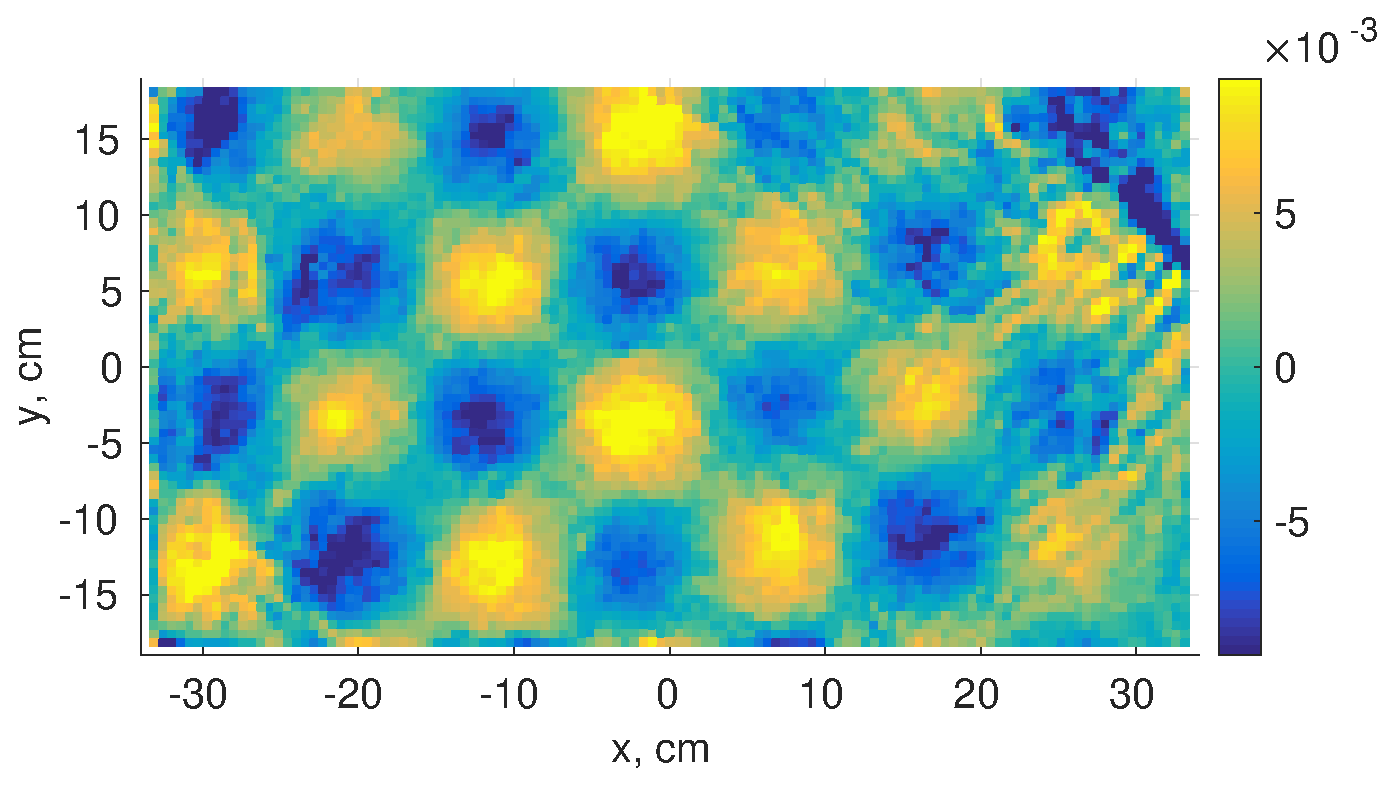
\includegraphics[width=.9\linewidth]{part6/vort0p5cm.eps} \\ а)}
 \end{minipage}
 \hfill
 \begin{minipage}[ht]{0.35\linewidth}
  \center
  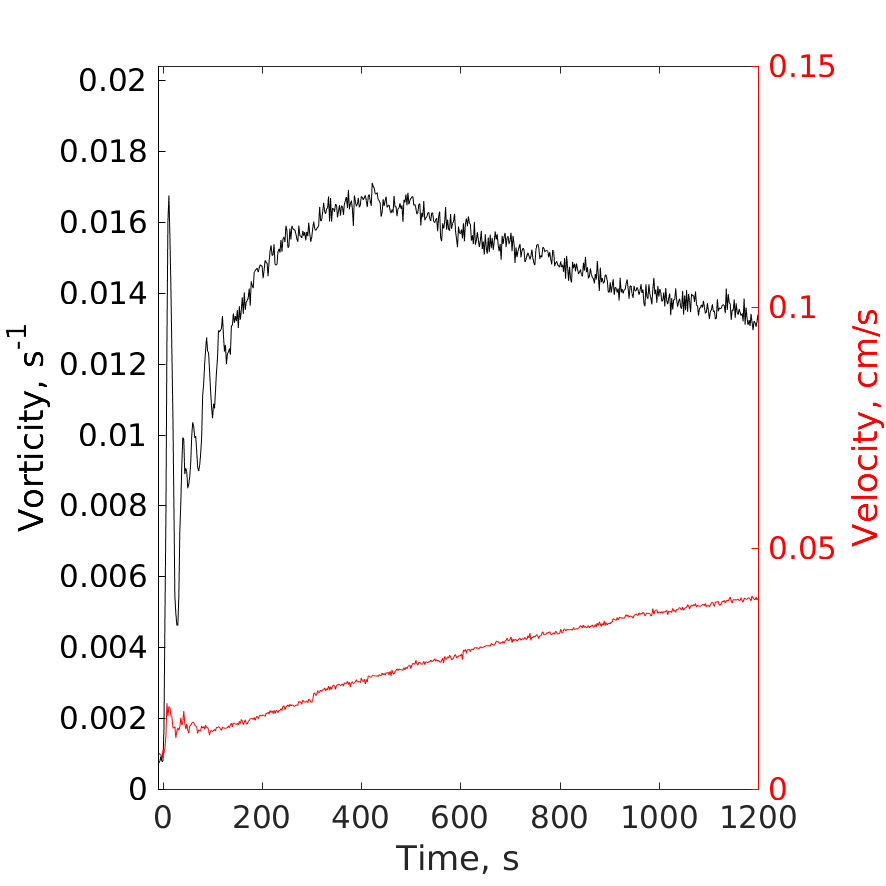
\includegraphics [width=1\linewidth]{part6/long_30mV_vel.jpg} \\ б)
 \end{minipage}

  \caption{а) Фрагмент 40х70 см$^2$ поля вертикальной завихренности в горизонтальном слое на глубине 0.5 см.
  б) Зависимость амплитуды завихренности решетки вихрей и скорости крупномасштабного течения от времени для амплитуд накачки  30 мВ на глубине 1 см.}
 \label{img:underLong} 
\end{figure}


\begin{figure}[ht]
  \center{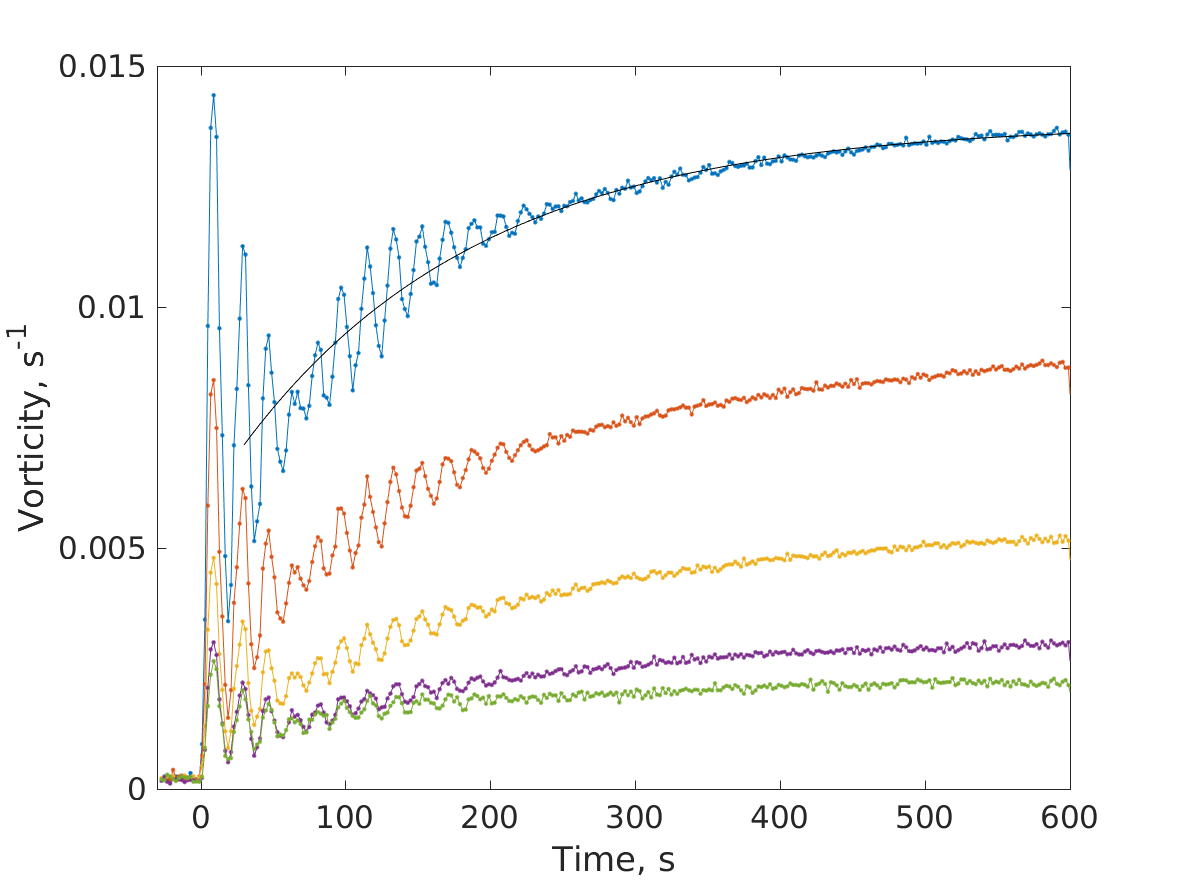
\includegraphics[width=.9\linewidth]{part6/5deeps.jpg} }

 \caption{Зависимость амплитуды завихренности решетки вихрей от времени, на глубинах 0.5~см, 1.25~см, 2.0~см, 2.75~см, 3.5~см. Черная кривая соответствует зависимости $1.4 \cdot 10^{-2} - 8 \cdot 10^{-3} e^{-t/165}$.}
 \label{img:5deeps} 
\end{figure}


На рисунке~\ref{img:5deeps} показана эволюция амплитуды решетки вихрей со временем после включения накачки. Пять кривых на рисунке соответствуют измерения на глубинах 0.5 см, 1.25 см, 2.0 см, 2.75 см, 3.5 см. Черной кривой показана зависимость $1.4 \cdot 10^{-2} - 8 \cdot 10^{-3} e^{-t/165}$.  Колебания завихренности на начальном участке объясняются колебанием амплитуд волн, связанными с переходными процессами. Т.е. на глубине 0.5 см завихренность росла с характерным временем 165 с. Оценка характерного времени роста завихренности для других глубин так же дают характерные времена около 200 с.


\begin{figure}[ht]
 \center
 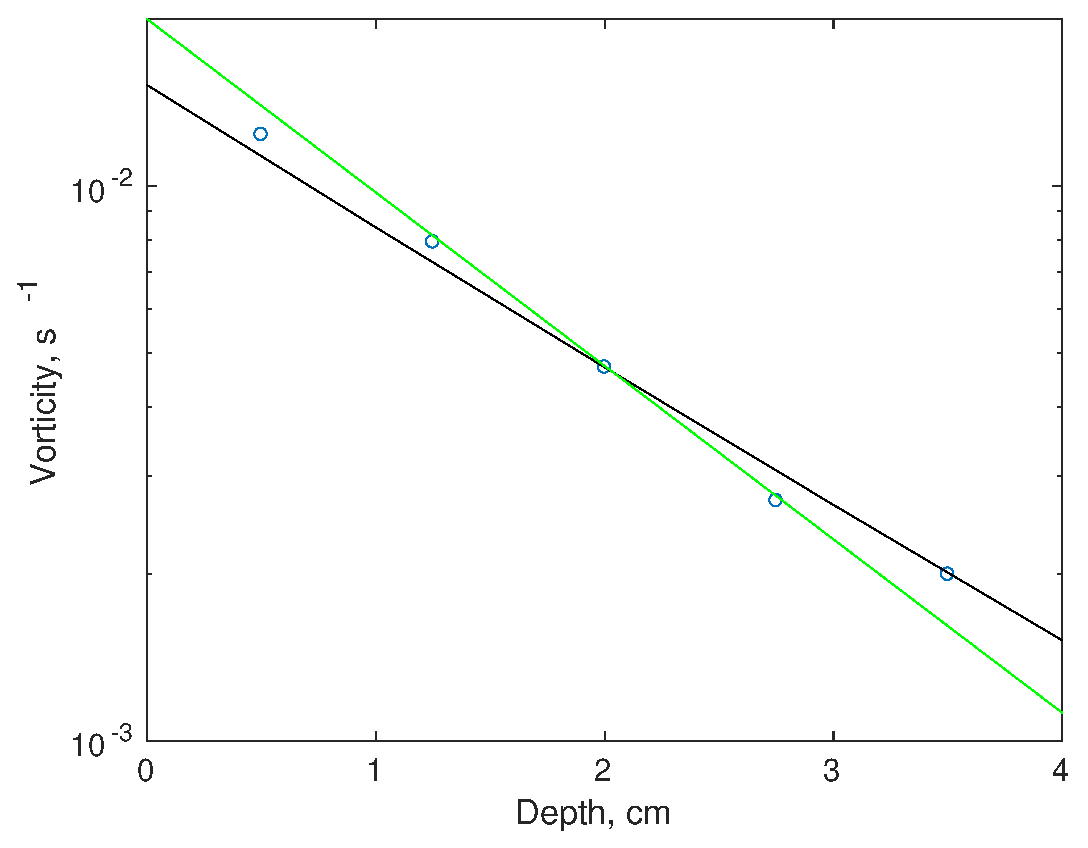
\includegraphics [width=.5\linewidth] {part6/depth.eps}
 \caption{Зависимость амплитуды завихренности решетки вихрей от глубины. Черная линия соответствует зависимости $6.3 \cdot 10^{-3} (e^{-2kh}+\sqrt{2}e^{-\sqrt{2}kh})$, зеленая прямая - $2 \cdot 10^{-2} e^{-2kh}$}
 \label{img:depth} 
\end{figure}

Также стоит отметить, что крупномасштабные вихревые течений, развивающиеся на поверхности воды сносят вихри и деформируют решетку завихренности. На рисунке~\ref{img:underLong}б показан график зависимости амплитуды решетки вихрей и средней скорости крупномасштабного течения от времени после включения накачки. На нем видно, что после 400-ой секунды завихренность решетки вихрей перестает расти и начинает уменьшаться. Начинает это происходить при характерной средней скорости крупномасштабного течения в $5 \cdot 10^{-3}$ см/с.

На рисунке~\ref{img:depth} показан график зависимости завихренности, усредненной в промежутке времени от 500 до 600 секунд после включения накачки, от глубины. Сплошные линии соответствуют зависимостям $e^{-2kh}+\sqrt{2}e^{-\sqrt{2}kh}$ и - $2 \cdot 10^{-2} e^{-2kh}$ , где k = 0.36~см$^{-1}$. Как видно из рисунка разброс экспериментальных точек не позволяют однозначно соотнести их с одной или другой экспоненциальной зависимостью. Стоит отметить, что снос завихренности решетки вихрей из-за развития крупномасштабных течений так же уменьшает значение завихренно­сти решетки вихрей, продиффундировавшей из вязкого подслоя. Этим, в свою очередь, можно объяснять расхождение экспериментальных данных с теоретической зависимостью

Таким образом можно сделать выводы:

-экспериментально показано, что распределение по глубине амплитуды завихренности решетки вихрей можно описать экспоненциальной зависимостью $e^{-2kh}$, где k — волновой вектор возбуждаемой решетки, а h — глубина слоя жидкости. 

-экспериментально оценено характерное время $\tau \approx 200$ с проникновения завихренности решетки вихрей из вязкого подслоя в объем. 

-экспериментально показано, что наличие крупномасштабных вихрей приводит к "сносу"{} завихренности, проникающей в объем из вязкого подслоя. Показано, что крупномасштабные течения с характерной скоростью $5 \cdot 10^{-3}$ см/c приводят к существенной деградации завихренности решетки вихрей с характерным размером вихря 8 см.


В \underline{\textbf{заключении}} приведены основные результаты работы, которые заключаются в следующем.

В диссертационной работе выполнены экспериментальные исследования капиллярной волновой турбулентности на поверхности жидкого водорода и воды, а так же исследования генерации вихревого движение на свободной поверхности жидкости волнами, движущимися под углом друг к другу.

1. Впервые наблюден переход от степенного распределения энергии в инерционном интервале спектра Колмогорова-Захарова к "квазипланковскому"{} распределению $\omega^{-s}e^{-\omega/\omega_d}$ в области диссипации для капиллярной турбулентности при накачке в полосе частот. Экспоненциальная зависимость энергии от частоты в области диссипации $\omega/\omega_d \gg 1$ соответствует теоретическому ожиданию и качественно соответствует численным вычислениям \cite{Ryzhenkova1990}. Граница вязкого затухания $\omega_d$ растет с увеличением амплитуды накачки и зависит от средней высоты волны $\eta_0$ на частоте накачки как $\omega_d \sim \eta^{0.85 \pm 0.05}$. Однако наблюденная зависимость отличается от теоретически ожидаемой, показатель степени почти в три раза меньше, чем предсказанное значение.

2. Экспериментально показано, что при возбуждении турбулентного состояния на поверхности воды монохроматической или широкополосной накачкой частота высокочастотного края инерционного интервала и характерная частота экспоненциального затухания энергии в диссипативной области отличаются в несколько раз друг от друга и качественно одинаково повышаются с ростом амплитуды накачки по степенному закону с показателем степени, близким к теоретически оцененному значению для случая монохроматического возбуждения. В случае возбуждения широкополосной накачкой наблюдается значительное расхождение между экспериментальными и теоретически оцененными значениями показателя $\beta$.

3. Открыт новый механизм генерации вихревого движения поверхностными волнами распространяющимися под углом друг к другу. Показано, что генерация вихревого движения на поверхности жидкости не является специфической чертой волн Фарадея.

4. Экспериментально подтверждена теоретическая модель генерации вихревого движения перпендикулярными волнами на поверхности воды как для капиллярных, так и для гравитационных волн. Экспериментально показано, что амплитуда завихренности решетки вихрей на поверхности воды квадратично зависит от амплитуды волн накачки, и зависит как $sin(\psi)$ от разности фаз $\psi$ между стоячими волнами в перпендикулярных направлениях. 

5. Экспериментально показано, что в объеме воды решетка вихрей сохраняет структуру и зависимость амплитуды завихренности от глубины близка к экспоненциальному закону $e^{-2kh}$, где k — волновой вектор возбуждаемой решетки, а h — глубина слоя жидкости. 
Экспериментально оценено характерное время проникновения завихренности решетки вихрей в объем при накачке двумя перпендикулярными волнами на частоте 3 Гц в 200 секунд.

6. Экспериментально показано, что наличие крупномасштабных вихрей приводит к сносу решетки вихрей. Оценены характерные скорости крупномасштабных течений приводящие к существенной деградации вихрей, формирующих решетку.


\clearpage 
\chapter*{Публикации автора}	% Добавляем его в оглавление
%
%
[F1] Brazhnikov M.Yu., Abdurakhimov L.V., Filatov S.V., Levchenko A.A., "Quasi-Planck"{} spectra of capillary turbulence on the surface of liquid hydrogen // JETP Lett. 2011.V. 93. P. 34.

[F2] Л.В. Абдурахимов, М.Ю. Бражников, А.А. Левченко, И.А. Ремизов, С.В. Филатов, "Турбулентный капиллярный каскад вблизи края инерционного интервала на поверхности квантовой жидкости"{}, Письма в ЖЭТФ, том 95 вып. 12, с. 751-760 (2012)

[F3] Л.В. Абдурахимов, М.Ю. Бражников, А.А. Левченко, И.А. Ремизов, С.В. Филатов, "Кинетическая и дискретная турбулентность на поверхности квантовой жидкости"{}, УФН, том 182, 8, с. 879 (2012)

[F4] С.В. Филатов, М.Ю. Бражников, А.А. Левченко, "Метод пространственной регистрации волн на поверхности прозрачной жидкости"{}, ПТЭ, 1, с. 107-112, (2014)

[F5] С.В. Филатов, М.Ю. Бражников, А.А. Левченко, "Формирование вихревого течения волнами на поверхности жидкости"{}, Письма в ЖЭТФ, том 102, вып. 7, с. 486-490 (2015)

[F6] S.V. Filatov, V.M. Parfenyev, S.S. Vergeles, M.Yu. Brazhnikov, A.A. Levchenko, V.V. Lebedev, "Nonlinear Generation of Vorticity by Surface Waves"{}, Physical Review Letters, 116, 054501 (2016)

[F7]. С.В. Филатов, М.Ю. Бражников, А.А. Левченко,  А.М. Лихтер, "Турбулентность в системе капиллярных волн на поверхности воды"{}, Поверхность, 10, с. 69-76 (2016)

[F8] С.В. Филатов, С.А. Алиев, А.А. Левченко, Д.А. Храмов, "Генерация вихрей гравитационными волнами на поверхности воды"{}, Письма в ЖЭТФ, том 104, вып.  10, с. 714-720 (2016)

%\input{common/concl}
\clearpage 

\bibliographystyle{BibTeX-Styles/ugost2008}
\bibliography{Synopsis/reference}

%\newpage
%При использовании пакета \verb!biblatex! список публикаций автора по теме
%диссертации формируется в разделе <<\publications>>\ файла
%\verb!../common/characteristic.tex!  при помощи команды \verb!\nocite! 

%\ifdefmacro{\microtypesetup}{\microtypesetup{protrusion=false}}{} % не рекомендуется применять пакет микротипографики к автоматически генерируемому списку литературы

%\ifnumequal{\value{bibliosel}}{0}{% Встроенная реализация с загрузкой файла через движок bibtex8
%  \renewcommand{\refname}{\large \authorbibtitle}
%  \nocite{*}
%  \insertbiblioauthor           % Подключаем Bib-базы
  %\insertbiblioother   % !!! bibtex не умеет работать с несколькими библиографиями !!!
%}{% Реализация пакетом biblatex через движок biber
%  \insertbiblioauthor           % Вывод всех работ автора
%  \insertbiblioauthorgrouped    % Вывод всех работ автора, сгруппированных по источникам
%  \insertbiblioauthorimportant  % Вывод наиболее значимых работ автора (определяется в файле characteristic во второй section)
%  \insertbiblioother            % Вывод списка литературы, на которую ссылались в тексте автореферата
%}
%\ifdefmacro{\microtypesetup}{\microtypesetup{protrusion=true}}{}

